% tables.tex -- public copy made by paper/deposit/build_release.py from the working manuscript.
% Every line that prints a number ends with a comment "% src: ..." that names the stored file and the key the
% number comes from; paper/check_numbers.py reads these comments (its header explains their forms) and
% docs/NUMBERS_TO_FILES.tsv of the package lists the files. Comment-only lines of the working manuscript (notes
% for the author) are not part of this copy; nothing that is printed differs.
\documentclass[aps,prx,onecolumn,10pt,nofootinbib,longbibliography,floatfix]{revtex4-2}

\usepackage[T1]{fontenc}
\usepackage{lmodern}
\usepackage{amsmath,amssymb,amsthm}
\usepackage{bm}
\usepackage{graphicx}
\usepackage{longtable}
\usepackage{booktabs}
\usepackage{xcolor}
\usepackage{pifont}
\usepackage{needspace}
\usepackage[colorlinks=true,linkcolor=blue!50!black,citecolor=blue!50!black,urlcolor=blue!50!black]{hyperref}

\graphicspath{{figures/}}
\setlength{\LTcapwidth}{\textwidth}
\raggedbottom
\renewcommand{\thesection}{A\arabic{section}}
\renewcommand{\thesubsection}{\thesection.\arabic{subsection}}
\renewcommand{\theequation}{S\arabic{equation}}
\renewcommand{\thefigure}{A\arabic{figure}}
\renewcommand{\thetable}{A\arabic{table}}

\newtheorem{theorem}{Theorem}
\newtheorem{proposition}{Proposition}
\renewcommand{\theproposition}{S\arabic{proposition}}
\newtheorem{lemma}{Lemma}
\renewcommand{\thelemma}{S\arabic{lemma}}
\theoremstyle{remark}
\newtheorem*{remark}{Remark}

\newcommand{\Jz}{J_z}
\newcommand{\ms}{m_s}
\newcommand{\Czz}{\bar C_{zz}}
\newcommand{\Ctwo}{\bar C_{2}}
\newcommand{\de}{\delta e}
\newcommand{\des}{\delta e^{*}}
\newcommand{\W}{\mathcal{W}}
\newcommand{\Tr}{\operatorname{Tr}}
\newcommand{\GS}{\mathrm{GS}}
\newcommand{\todo}[1]{\textcolor{red}{[TODO: #1]}}


\begin{document}

\title{Ancillary tables for ``What a sample's energy certifies about quantum-generated labels''}
\author{Nicol\'as Bonilla Vargas}
\affiliation{Universidad Nacional de Colombia, Bogot\'a, Colombia}
\affiliation{SRH University, Munich, Germany}
\affiliation{Daita AI, Munich, Germany}
\maketitle

\noindent This file holds the long tables of the certification map and of the emulation that the Supplemental
Material summarizes, and two extended figures. Every table is generated by \texttt{figures/make\_sm\_tables.py}
from the deposited outputs (the map tables are also checked cell by cell against the deposited Markdown tables:
2145 cells, no difference); every figure by the script named in \texttt{figures/FIGURES\_README.md}. Numbers are % src: file:paper/figures/FIGURES_README.md (2145)
rounded to three significant digits (two for robustness fractions); the deposit keeps full precision. Rows dropped by
the declared cost rule ($n=115$ local labels except $Z_{\rm bulk}$ at $\Jz=4.0$; $n=115$ at $\Jz=3.2,3.4$) are
absent. Energies are in units of the exchange coupling; $\tau=0.06|o_\GS|$; ``certified'' means that the window is % src: def:phase3/full_runs/map/DECLARATION.md (tau = 0.06|O_GS|)
at most $\tau$ wide under the windows of Supplemental Sec.~S3, so that the label is within $\tau$ ($6\%$ of % src: def:phase3/full_runs/map/DECLARATION.md (6 %)
$|o_\GS|$) of the ground-state value; only the window midpoint is within $\tau/2$. The $\ms$ statuses assume
in-sector states.

\section{Certification map: full tables}
\def\SMcap{Widths of the information limit at $n=57$. Each block is one label and each row one computed coupling
$\Jz$ ($^\dagger$: out-of-distribution point, where no energy is published and the conditional floor
$\epsilon_{\rm dig}=0.012\,n$ is used). Read along a row: the energy window always contains an interval at least % src: def:phase3/full_runs/map/DECLARATION.md (0.012)
$w_{\rm in}$ wide, and DMRG-referenced bounds show it is at most $w_{\rm out}$ wide. $o_\GS$: ground-state value (bond
dimension $320$); $\epsilon_{\rm dig}=E_{\rm dig}-E_0$: the dataset's total energy error, read from its figures % src: file:phase3/full_runs/map/RESULTS.md; def:phase3/full_runs/map/DECLARATION.md
(reading 1); $w_{\rm in}$: rigorous inner width at the lower window $E_{\rm lo}$ (hull of the stored sector states and
two-state mixtures); $w_{\rm pure}$: the same with single stored pure states only; $w_{\rm out}$: outer width at the
upper window $E_{\rm up}$; last column: the map value, the outer width at the dataset's energy in units of
$\tau=0.06|o_\GS|$. Bold $\Jz$: certified, i.e.\ $w_{\rm out}(E_{\rm up})\le\tau$.}\def\SMlab{tab:map_widths_n57} % src: def:phase3/full_runs/map/DECLARATION.md (tau = 0.06|O_GS|; n = 57)
% generated by figures/make_sm_tables.py from phase3/full_runs/map/laptop_analysis/summary_map.json (rows with n = 57); same values as phase3/full_runs/map/laptop_analysis/tables_map.md -- do not edit
{\footnotesize\setlength{\tabcolsep}{5pt}\renewcommand{\arraystretch}{1.3}
\needspace{532pt}
\begin{longtable}{lcccccc}
\caption{\SMcap}\label{\SMlab}\\
\toprule
 & & & \multicolumn{2}{c}{lower window $E_{\rm lo}$} & upper window $E_{\rm up}$ & dataset's energy $E_{\rm dig}$ \\ \cmidrule(lr){4-5}\cmidrule(lr){6-6}\cmidrule(l){7-7}
$J_z$ & $o_{\rm GS}$ & $\epsilon_{\rm dig}$ & $w_{\rm in}$ (rigorous) & $w_{\rm pure}$ & $w_{\rm out}$ & $w_{\rm out}/\tau$ \\
\midrule
\multicolumn{7}{@{}l}{\textbf{Staggered magnetization $m_s$}}\\
1.1\rlap{$^{\dagger}$} & \phantom{$-$}0.595 & 0.684\phantom{0} & 0.501\phantom{0} & 0.485\phantom{0} & 0.619\phantom{0} & 15.8\phantom{00} \\
1.2\rlap{$^{\dagger}$} & \phantom{$-$}0.640 & 0.684\phantom{0} & 0.462\phantom{0} & 0.439\phantom{0} & 0.574\phantom{0} & 13.6\phantom{00} \\
1.3\rlap{$^{\dagger}$} & \phantom{$-$}0.680 & 0.684\phantom{0} & 0.424\phantom{0} & 0.383\phantom{0} & 0.530\phantom{0} & 11.8\phantom{00} \\
1.4\rlap{$^{\dagger}$} & \phantom{$-$}0.714 & 0.684\phantom{0} & 0.388\phantom{0} & 0.336\phantom{0} & 0.487\phantom{0} & 10.3\phantom{00} \\
1.6 & \phantom{$-$}0.770 & 0.624\phantom{0} & 0.308\phantom{0} & 0.305\phantom{0} & 0.398\phantom{0} & \phantom{0}7.61\phantom{0} \\
1.8 & \phantom{$-$}0.812 & 0.513\phantom{0} & 0.232\phantom{0} & 0.210\phantom{0} & 0.294\phantom{0} & \phantom{0}5.44\phantom{0} \\
2.0 & \phantom{$-$}0.845 & 0.435\phantom{0} & 0.181\phantom{0} & 0.166\phantom{0} & 0.228\phantom{0} & \phantom{0}4.07\phantom{0} \\
2.5 & \phantom{$-$}0.897 & 0.249\phantom{0} & 0.0951 & 0.0933 & 0.118\phantom{0} & \phantom{0}2.00\phantom{0} \\
3.0 & \phantom{$-$}0.927 & 0.161\phantom{0} & 0.0572 & 0.0566 & 0.0708 & \phantom{0}1.16\phantom{0} \\
3.2 & \phantom{$-$}0.936 & 0.145\phantom{0} & 0.0490 & 0.0477 & 0.0607 & \phantom{0}0.980 \\
3.3 & \phantom{$-$}0.940 & 0.153\phantom{0} & 0.0480 & 0.0453 & 0.0595 & \phantom{0}0.956 \\
\textbf{3.4} & \phantom{$-$}0.943 & 0.140\phantom{0} & 0.0438 & 0.0427 & 0.0542 & \phantom{0}0.871 \\
\textbf{3.6} & \phantom{$-$}0.949 & 0.122\phantom{0} & 0.0374 & 0.0368 & 0.0461 & \phantom{0}0.738 \\
\textbf{4.0} & \phantom{$-$}0.959 & 0.0985 & 0.0285 & 0.0284 & 0.0351 & \phantom{0}0.558 \\
\textbf{4.5} & \phantom{$-$}0.967 & 0.0771 & 0.0210 & 0.0204 & 0.0259 & \phantom{0}0.407 \\
\textbf{5.0} & \phantom{$-$}0.973 & 0.0575 & 0.0154 & 0.0151 & 0.0190 & \phantom{0}0.297 \\
\textbf{5.5} & \phantom{$-$}0.978 & 0.0527 & 0.0128 & 0.0125 & 0.0157 & \phantom{0}0.244 \\
\textbf{6.0} & \phantom{$-$}0.981 & 0.0517 & 0.0111 & 0.0108 & 0.0136 & \phantom{0}0.211 \\
\multicolumn{7}{@{}l}{\textbf{Mean nearest-neighbour correlation $\bar C_{zz}$}}\\
1.1\rlap{$^{\dagger}$} & $-$0.643 & 0.684\phantom{0} & 0.298\phantom{0} & 0.293\phantom{0} & 0.362\phantom{0} & \phantom{0}8.62\phantom{0} \\
1.2\rlap{$^{\dagger}$} & $-$0.675 & 0.684\phantom{0} & 0.286\phantom{0} & 0.285\phantom{0} & 0.348\phantom{0} & \phantom{0}7.88\phantom{0} \\
1.3\rlap{$^{\dagger}$} & $-$0.705 & 0.684\phantom{0} & 0.273\phantom{0} & 0.271\phantom{0} & 0.333\phantom{0} & \phantom{0}7.22\phantom{0} \\
1.4\rlap{$^{\dagger}$} & $-$0.731 & 0.684\phantom{0} & 0.260\phantom{0} & 0.258\phantom{0} & 0.317\phantom{0} & \phantom{0}6.62\phantom{0} \\
1.6 & $-$0.777 & 0.624\phantom{0} & 0.223\phantom{0} & 0.221\phantom{0} & 0.278\phantom{0} & \phantom{0}5.35\phantom{0} \\
1.8 & $-$0.813 & 0.513\phantom{0} & 0.181\phantom{0} & 0.179\phantom{0} & 0.221\phantom{0} & \phantom{0}4.16\phantom{0} \\
2.0 & $-$0.842 & 0.435\phantom{0} & 0.149\phantom{0} & 0.148\phantom{0} & 0.183\phantom{0} & \phantom{0}3.31\phantom{0} \\
2.5 & $-$0.892 & 0.249\phantom{0} & 0.0869 & 0.0859 & 0.107\phantom{0} & \phantom{0}1.83\phantom{0} \\
3.0 & $-$0.922 & 0.161\phantom{0} & 0.0554 & 0.0542 & 0.0680 & \phantom{0}1.12\phantom{0} \\
3.2 & $-$0.931 & 0.145\phantom{0} & 0.0482 & 0.0473 & 0.0593 & \phantom{0}0.966 \\
\bottomrule
\multicolumn{7}{r@{}}{\textit{continued on next page}}\\
\end{longtable}
\needspace{474pt}
\begin{center}\begin{tabular}{lcccccc}
\multicolumn{7}{@{}l}{\textit{Table \thetable\ (continued)}}\\
\toprule
 & & & \multicolumn{2}{c}{lower window $E_{\rm lo}$} & upper window $E_{\rm up}$ & dataset's energy $E_{\rm dig}$ \\ \cmidrule(lr){4-5}\cmidrule(lr){6-6}\cmidrule(l){7-7}
$J_z$ & $o_{\rm GS}$ & $\epsilon_{\rm dig}$ & $w_{\rm in}$ (rigorous) & $w_{\rm pure}$ & $w_{\rm out}$ & $w_{\rm out}/\tau$ \\
\midrule
\multicolumn{7}{@{}l}{\textbf{Mean nearest-neighbour correlation $\bar C_{zz}$ \textmd{\textit{(continued)}}}}\\
3.3 & $-$0.935 & 0.153\phantom{0} & 0.0475 & 0.0465 & 0.0584 & \phantom{0}0.948 \\
\textbf{3.4} & $-$0.938 & 0.140\phantom{0} & 0.0436 & 0.0427 & 0.0536 & \phantom{0}0.869 \\
\textbf{3.6} & $-$0.945 & 0.122\phantom{0} & 0.0376 & 0.0370 & 0.0461 & \phantom{0}0.744 \\
\textbf{4.0} & $-$0.955 & 0.0985 & 0.0292 & 0.0287 & 0.0358 & \phantom{0}0.571 \\
\textbf{4.5} & $-$0.964 & 0.0771 & 0.0219 & 0.0215 & 0.0269 & \phantom{0}0.424 \\
\textbf{5.0} & $-$0.970 & 0.0575 & 0.0162 & 0.0160 & 0.0200 & \phantom{0}0.312 \\
\textbf{5.5} & $-$0.975 & 0.0527 & 0.0135 & 0.0134 & 0.0166 & \phantom{0}0.259 \\
\textbf{6.0} & $-$0.979 & 0.0517 & 0.0118 & 0.0116 & 0.0145 & \phantom{0}0.225 \\
\multicolumn{7}{@{}l}{\textbf{Mean next-nearest-neighbour correlation $\bar C_{2}$}}\\
1.1\rlap{$^{\dagger}$} & \phantom{$-$}0.426 & 0.684\phantom{0} & 0.455\phantom{0} & 0.449\phantom{0} & 0.549\phantom{0} & 19.8\phantom{00} \\
1.2\rlap{$^{\dagger}$} & \phantom{$-$}0.475 & 0.684\phantom{0} & 0.444\phantom{0} & 0.438\phantom{0} & 0.538\phantom{0} & 17.4\phantom{00} \\
1.3\rlap{$^{\dagger}$} & \phantom{$-$}0.521 & 0.684\phantom{0} & 0.429\phantom{0} & 0.421\phantom{0} & 0.521\phantom{0} & 15.3\phantom{00} \\
1.4\rlap{$^{\dagger}$} & \phantom{$-$}0.563 & 0.684\phantom{0} & 0.413\phantom{0} & 0.403\phantom{0} & 0.501\phantom{0} & 13.6\phantom{00} \\
1.6 & \phantom{$-$}0.635 & 0.624\phantom{0} & 0.359\phantom{0} & 0.356\phantom{0} & 0.446\phantom{0} & 10.5\phantom{00} \\
1.8 & \phantom{$-$}0.693 & 0.513\phantom{0} & 0.294\phantom{0} & 0.290\phantom{0} & 0.359\phantom{0} & \phantom{0}7.92\phantom{0} \\
2.0 & \phantom{$-$}0.740 & 0.435\phantom{0} & 0.243\phantom{0} & 0.241\phantom{0} & 0.299\phantom{0} & \phantom{0}6.16\phantom{0} \\
2.5 & \phantom{$-$}0.821 & 0.249\phantom{0} & 0.143\phantom{0} & 0.143\phantom{0} & 0.176\phantom{0} & \phantom{0}3.27\phantom{0} \\
3.0 & \phantom{$-$}0.871 & 0.161\phantom{0} & 0.0917 & 0.0895 & 0.113\phantom{0} & \phantom{0}1.97\phantom{0} \\
3.3 & \phantom{$-$}0.892 & 0.153\phantom{0} & 0.0788 & 0.0772 & 0.0969 & \phantom{0}1.65\phantom{0} \\
3.6 & \phantom{$-$}0.908 & 0.122\phantom{0} & 0.0625 & 0.0614 & 0.0766 & \phantom{0}1.29\phantom{0} \\
4.0 & \phantom{$-$}0.925 & 0.0985 & 0.0485 & 0.0478 & 0.0596 & \phantom{0}0.978 \\
\textbf{4.5} & \phantom{$-$}0.940 & 0.0771 & 0.0364 & 0.0359 & 0.0447 & \phantom{0}0.723 \\
\textbf{5.0} & \phantom{$-$}0.951 & 0.0575 & 0.0270 & 0.0267 & 0.0332 & \phantom{0}0.531 \\
\textbf{5.5} & \phantom{$-$}0.959 & 0.0527 & 0.0226 & 0.0223 & 0.0276 & \phantom{0}0.439 \\
\textbf{6.0} & \phantom{$-$}0.966 & 0.0517 & 0.0197 & 0.0194 & 0.0242 & \phantom{0}0.381 \\
\multicolumn{7}{@{}l}{\textbf{Bulk site $Z_{\rm bulk}$ (degree 3)}}\\
1.1\rlap{$^{\dagger}$} & $-$0.584 & 0.684\phantom{0} & 1.45\phantom{00} & 0.724\phantom{0} & 1.78\phantom{00} & 47.5\phantom{00} \\
1.2\rlap{$^{\dagger}$} & $-$0.635 & 0.684\phantom{0} & 1.39\phantom{00} & 0.643\phantom{0} & 1.69\phantom{00} & 41.2\phantom{00} \\
1.3\rlap{$^{\dagger}$} & $-$0.678 & 0.684\phantom{0} & 1.31\phantom{00} & 0.568\phantom{0} & 1.60\phantom{00} & 36.3\phantom{00} \\
1.4\rlap{$^{\dagger}$} & $-$0.715 & 0.684\phantom{0} & 1.24\phantom{00} & 0.504\phantom{0} & 1.51\phantom{00} & 32.4\phantom{00} \\
1.6 & $-$0.772 & 0.624\phantom{0} & 1.04\phantom{00} & 1.04\phantom{00} & 1.31\phantom{00} & 25.3\phantom{00} \\
1.8 & $-$0.815 & 0.513\phantom{0} & 0.831\phantom{0} & 0.821\phantom{0} & 1.03\phantom{00} & 19.2\phantom{00} \\
2.0 & $-$0.847 & 0.435\phantom{0} & 0.675\phantom{0} & 0.623\phantom{0} & 0.844\phantom{0} & 15.1\phantom{00} \\
\bottomrule
\multicolumn{7}{r@{}}{\textit{continued on next page}}\\
\end{tabular}\end{center}
\needspace{383pt}
\begin{center}\begin{tabular}{lcccccc}
\multicolumn{7}{@{}l}{\textit{Table \thetable\ (continued)}}\\
\toprule
 & & & \multicolumn{2}{c}{lower window $E_{\rm lo}$} & upper window $E_{\rm up}$ & dataset's energy $E_{\rm dig}$ \\ \cmidrule(lr){4-5}\cmidrule(lr){6-6}\cmidrule(l){7-7}
$J_z$ & $o_{\rm GS}$ & $\epsilon_{\rm dig}$ & $w_{\rm in}$ (rigorous) & $w_{\rm pure}$ & $w_{\rm out}$ & $w_{\rm out}/\tau$ \\
\midrule
\multicolumn{7}{@{}l}{\textbf{Bulk site $Z_{\rm bulk}$ (degree 3) \textmd{\textit{(continued)}}}}\\
2.5 & $-$0.899 & 0.249\phantom{0} & 0.384\phantom{0} & 0.382\phantom{0} & 0.479\phantom{0} & \phantom{0}8.10\phantom{0} \\
3.0 & $-$0.929 & 0.161\phantom{0} & 0.242\phantom{0} & 0.241\phantom{0} & 0.301\phantom{0} & \phantom{0}4.94\phantom{0} \\
3.3 & $-$0.941 & 0.153\phantom{0} & 0.206\phantom{0} & 0.196\phantom{0} & 0.258\phantom{0} & \phantom{0}4.16\phantom{0} \\
3.6 & $-$0.950 & 0.122\phantom{0} & 0.163\phantom{0} & 0.159\phantom{0} & 0.203\phantom{0} & \phantom{0}3.25\phantom{0} \\
4.0 & $-$0.959 & 0.0985 & 0.126\phantom{0} & 0.125\phantom{0} & 0.157\phantom{0} & \phantom{0}2.50\phantom{0} \\
4.5 & $-$0.968 & 0.0771 & 0.0940 & 0.0915 & 0.118\phantom{0} & \phantom{0}1.86\phantom{0} \\
5.0 & $-$0.974 & 0.0575 & 0.0701 & 0.0676 & 0.0879 & \phantom{0}1.37\phantom{0} \\
5.5 & $-$0.978 & 0.0527 & 0.0579 & 0.0572 & 0.0729 & \phantom{0}1.14\phantom{0} \\
6.0 & $-$0.982 & 0.0517 & 0.0498 & 0.0460 & 0.0636 & \phantom{0}0.991 \\
\multicolumn{7}{@{}l}{\textbf{Boundary site $Z_{\rm bdry}$ (degree 1)}}\\
1.1\rlap{$^{\dagger}$} & \phantom{$-$}0.708 & 0.684\phantom{0} & 1.65\phantom{00} & 0.431\phantom{0} & 2.00\phantom{00} & 44.8\phantom{00} \\
1.2\rlap{$^{\dagger}$} & \phantom{$-$}0.736 & 0.684\phantom{0} & 1.58\phantom{00} & 0.408\phantom{0} & 1.96\phantom{00} & 41.7\phantom{00} \\
1.3\rlap{$^{\dagger}$} & \phantom{$-$}0.762 & 0.684\phantom{0} & 1.51\phantom{00} & 0.378\phantom{0} & 1.91\phantom{00} & 38.6\phantom{00} \\
1.4\rlap{$^{\dagger}$} & \phantom{$-$}0.786 & 0.684\phantom{0} & 1.43\phantom{00} & 0.345\phantom{0} & 1.84\phantom{00} & 35.9\phantom{00} \\
1.6 & \phantom{$-$}0.826 & 0.624\phantom{0} & 1.23\phantom{00} & 0.312\phantom{0} & 1.65\phantom{00} & 29.4\phantom{00} \\
1.8 & \phantom{$-$}0.857 & 0.513\phantom{0} & 1.02\phantom{00} & 1.01\phantom{00} & 1.30\phantom{00} & 22.8\phantom{00} \\
2.0 & \phantom{$-$}0.882 & 0.435\phantom{0} & 0.818\phantom{0} & 0.769\phantom{0} & 1.06\phantom{00} & 18.0\phantom{00} \\
2.5 & \phantom{$-$}0.922 & 0.249\phantom{0} & 0.450\phantom{0} & 0.448\phantom{0} & 0.577\phantom{0} & \phantom{0}9.38\phantom{0} \\
3.0 & \phantom{$-$}0.945 & 0.161\phantom{0} & 0.275\phantom{0} & 0.271\phantom{0} & 0.351\phantom{0} & \phantom{0}5.56\phantom{0} \\
3.3 & \phantom{$-$}0.954 & 0.153\phantom{0} & 0.234\phantom{0} & 0.231\phantom{0} & 0.300\phantom{0} & \phantom{0}4.69\phantom{0} \\
3.6 & \phantom{$-$}0.962 & 0.122\phantom{0} & 0.182\phantom{0} & 0.173\phantom{0} & 0.232\phantom{0} & \phantom{0}3.61\phantom{0} \\
4.0 & \phantom{$-$}0.969 & 0.0985 & 0.139\phantom{0} & 0.138\phantom{0} & 0.176\phantom{0} & \phantom{0}2.73\phantom{0} \\
4.5 & \phantom{$-$}0.975 & 0.0771 & 0.103\phantom{0} & 0.0984 & 0.130\phantom{0} & \phantom{0}2.01\phantom{0} \\
5.0 & \phantom{$-$}0.980 & 0.0575 & 0.0753 & 0.0731 & 0.0951 & \phantom{0}1.46\phantom{0} \\
5.5 & \phantom{$-$}0.983 & 0.0527 & 0.0622 & 0.0601 & 0.0786 & \phantom{0}1.21\phantom{0} \\
6.0 & \phantom{$-$}0.986 & 0.0517 & 0.0540 & 0.0534 & 0.0689 & \phantom{0}1.05\phantom{0} \\
\bottomrule
\multicolumn{7}{r@{}}{\textit{continued on next page}}\\
\end{tabular}\end{center}
\needspace{474pt}
\begin{center}\begin{tabular}{lcccccc}
\multicolumn{7}{@{}l}{\textit{Table \thetable\ (continued)}}\\
\toprule
 & & & \multicolumn{2}{c}{lower window $E_{\rm lo}$} & upper window $E_{\rm up}$ & dataset's energy $E_{\rm dig}$ \\ \cmidrule(lr){4-5}\cmidrule(lr){6-6}\cmidrule(l){7-7}
$J_z$ & $o_{\rm GS}$ & $\epsilon_{\rm dig}$ & $w_{\rm in}$ (rigorous) & $w_{\rm pure}$ & $w_{\rm out}$ & $w_{\rm out}/\tau$ \\
\midrule
\multicolumn{7}{@{}l}{\textbf{One bulk edge $C_{zz}^{\rm edge}$}}\\
1.1\rlap{$^{\dagger}$} & $-$0.651 & 0.684\phantom{0} & 1.33\phantom{00} & 0.526\phantom{0} & 1.63\phantom{00} & 38.7\phantom{00} \\
1.2\rlap{$^{\dagger}$} & $-$0.686 & 0.684\phantom{0} & 1.28\phantom{00} & 0.484\phantom{0} & 1.56\phantom{00} & 35.0\phantom{00} \\
1.3\rlap{$^{\dagger}$} & $-$0.717 & 0.684\phantom{0} & 1.22\phantom{00} & 0.442\phantom{0} & 1.49\phantom{00} & 31.8\phantom{00} \\
1.4\rlap{$^{\dagger}$} & $-$0.745 & 0.684\phantom{0} & 1.16\phantom{00} & 0.404\phantom{0} & 1.42\phantom{00} & 29.1\phantom{00} \\
1.6 & $-$0.791 & 0.624\phantom{0} & 0.993\phantom{0} & 0.989\phantom{0} & 1.25\phantom{00} & 23.5\phantom{00} \\
1.8 & $-$0.827 & 0.513\phantom{0} & 0.799\phantom{0} & 0.789\phantom{0} & 0.996\phantom{0} & 18.3\phantom{00} \\
2.0 & $-$0.855 & 0.435\phantom{0} & 0.654\phantom{0} & 0.601\phantom{0} & 0.819\phantom{0} & 14.5\phantom{00} \\
2.5 & $-$0.902 & 0.249\phantom{0} & 0.377\phantom{0} & 0.374\phantom{0} & 0.470\phantom{0} & \phantom{0}7.92\phantom{0} \\
3.0 & $-$0.930 & 0.161\phantom{0} & 0.239\phantom{0} & 0.238\phantom{0} & 0.297\phantom{0} & \phantom{0}4.87\phantom{0} \\
3.3 & $-$0.942 & 0.153\phantom{0} & 0.204\phantom{0} & 0.194\phantom{0} & 0.255\phantom{0} & \phantom{0}4.11\phantom{0} \\
3.6 & $-$0.951 & 0.122\phantom{0} & 0.161\phantom{0} & 0.158\phantom{0} & 0.201\phantom{0} & \phantom{0}3.22\phantom{0} \\
4.0 & $-$0.960 & 0.0985 & 0.125\phantom{0} & 0.124\phantom{0} & 0.156\phantom{0} & \phantom{0}2.48\phantom{0} \\
4.5 & $-$0.968 & 0.0771 & 0.0934 & 0.0908 & 0.117\phantom{0} & \phantom{0}1.85\phantom{0} \\
5.0 & $-$0.974 & 0.0575 & 0.0697 & 0.0672 & 0.0874 & \phantom{0}1.37\phantom{0} \\
5.5 & $-$0.978 & 0.0527 & 0.0577 & 0.0569 & 0.0726 & \phantom{0}1.14\phantom{0} \\
6.0 & $-$0.982 & 0.0517 & 0.0497 & 0.0457 & 0.0634 & \phantom{0}0.988 \\
\multicolumn{7}{@{}l}{\textbf{One 12-site loop $Z_{\rm loop}$}}\\
1.1\rlap{$^{\dagger}$} & \phantom{$-$}0.384 & 0.684\phantom{0} & 1.51\phantom{00} & 0.899\phantom{0} & 1.79\phantom{00} & 73.9\phantom{00} \\
1.2\rlap{$^{\dagger}$} & \phantom{$-$}0.441 & 0.684\phantom{0} & 1.49\phantom{00} & 0.845\phantom{0} & 1.74\phantom{00} & 62.0\phantom{00} \\
1.3\rlap{$^{\dagger}$} & \phantom{$-$}0.493 & 0.684\phantom{0} & 1.44\phantom{00} & 0.759\phantom{0} & 1.68\phantom{00} & 53.3\phantom{00} \\
1.4\rlap{$^{\dagger}$} & \phantom{$-$}0.540 & 0.684\phantom{0} & 1.37\phantom{00} & 0.699\phantom{0} & 1.61\phantom{00} & 46.6\phantom{00} \\
1.6 & \phantom{$-$}0.619 & 0.624\phantom{0} & 1.20\phantom{00} & 1.18\phantom{00} & 1.45\phantom{00} & 35.8\phantom{00} \\
1.8 & \phantom{$-$}0.681 & 0.513\phantom{0} & 0.995\phantom{0} & 0.973\phantom{0} & 1.19\phantom{00} & 27.2\phantom{00} \\
2.0 & \phantom{$-$}0.730 & 0.435\phantom{0} & 0.832\phantom{0} & 0.811\phantom{0} & 1.00\phantom{00} & 21.3\phantom{00} \\
2.5 & \phantom{$-$}0.814 & 0.249\phantom{0} & 0.505\phantom{0} & 0.500\phantom{0} & 0.615\phantom{0} & 11.6\phantom{00} \\
3.0 & \phantom{$-$}0.866 & 0.161\phantom{0} & 0.327\phantom{0} & 0.325\phantom{0} & 0.399\phantom{0} & \phantom{0}7.04\phantom{0} \\
3.3 & \phantom{$-$}0.887 & 0.153\phantom{0} & 0.282\phantom{0} & 0.280\phantom{0} & 0.346\phantom{0} & \phantom{0}5.92\phantom{0} \\
3.6 & \phantom{$-$}0.904 & 0.122\phantom{0} & 0.224\phantom{0} & 0.218\phantom{0} & 0.274\phantom{0} & \phantom{0}4.62\phantom{0} \\
4.0 & \phantom{$-$}0.921 & 0.0985 & 0.175\phantom{0} & 0.172\phantom{0} & 0.214\phantom{0} & \phantom{0}3.54\phantom{0} \\
4.5 & \phantom{$-$}0.937 & 0.0771 & 0.132\phantom{0} & 0.130\phantom{0} & 0.161\phantom{0} & \phantom{0}2.62\phantom{0} \\
5.0 & \phantom{$-$}0.949 & 0.0575 & 0.0980 & 0.0958 & 0.120\phantom{0} & \phantom{0}1.93\phantom{0} \\
5.5 & \phantom{$-$}0.957 & 0.0527 & 0.0819 & 0.0801 & 0.100\phantom{0} & \phantom{0}1.60\phantom{0} \\
6.0 & \phantom{$-$}0.964 & 0.0517 & 0.0716 & 0.0703 & 0.0881 & \phantom{0}1.39\phantom{0} \\
\bottomrule
\end{tabular}\end{center}
}


\def\SMcap{Certification status and its robustness at $n=57$ (same rows as Table~\ref{tab:map_widths_n57}). Status
under reading 1 and the independent reading 2 of the dataset's energies: \emph{certified} if
$w_{\rm out}(E_{\rm up})\le\tau$, \emph{not certified} if $w_{\rm in}(E_{\rm lo})\ge\tau$, \emph{gray zone}
otherwise; out-of-distribution points ($^\dagger$) have no reading 2. Robustness fractions $f=\epsilon_\tau/\epsilon_{\rm
dig}$, with $\epsilon_\tau$ the energy error at which the inner ($f_{\rm in}$) or outer ($f_{\rm out}$) width equals
$\tau$: a ``not certified'' status holds for every true energy error above $f_{\rm in}\,\epsilon_{\rm dig}$, a
``certified'' one for every true error below $f_{\rm out}\,\epsilon_{\rm dig}$; $>$ marks a lower bound (the outer
width is still below $\tau$ at the end of the computed chain). $\epsilon_{\rm dig}/\Delta_{\rm in}$: energy error over
the in-sector gap. Last column: number of stored chain states of each sign. Bold $\Jz$: certified.}\def\SMlab{tab:map_status_n57} % src: def:phase3/full_runs/map/DECLARATION.md (n = 57)
% generated by figures/make_sm_tables.py from phase3/full_runs/map/laptop_analysis/summary_map.json (rows with n = 57); same values as phase3/full_runs/map/laptop_analysis/tables_map.md -- do not edit
{\footnotesize\setlength{\tabcolsep}{5pt}\renewcommand{\arraystretch}{1.3}
\needspace{532pt}
\begin{longtable}{lllcccc}
\caption{\SMcap}\label{\SMlab}\\
\toprule
 & \multicolumn{2}{c}{certification status} & \multicolumn{2}{c}{robustness fraction} & & \\ \cmidrule(lr){2-3}\cmidrule(lr){4-5}
$J_z$ & reading 1 & reading 2 & $f_{\rm in}$ & $f_{\rm out}$ & $\epsilon_{\rm dig}/\Delta_{\rm in}$ & chain states $+$\,/\,$-$ \\
\midrule
\multicolumn{7}{@{}l}{\textbf{Staggered magnetization $m_s$}}\\
1.1\rlap{$^{\dagger}$} & \ding{55}\,not certified & \textit{no reading} & \phantom{0}0.0045\phantom{0} & \phantom{0}0.0041\phantom{0000} & 0.98\phantom{00} & 8\,/\,8 \\
1.2\rlap{$^{\dagger}$} & \ding{55}\,not certified & \textit{no reading} & \phantom{0}0.0061\phantom{0} & \phantom{0}0.0059\phantom{0000} & 0.89\phantom{00} & 8\,/\,7 \\
1.3\rlap{$^{\dagger}$} & \ding{55}\,not certified & \textit{no reading} & \phantom{0}0.0083\phantom{0} & \phantom{0}0.0081\phantom{0000} & 0.81\phantom{00} & 8\,/\,7 \\
1.4\rlap{$^{\dagger}$} & \ding{55}\,not certified & \textit{no reading} & \phantom{0}0.011\phantom{00} & \phantom{0}0.011\phantom{00000} & 0.75\phantom{00} & 8\,/\,7 \\
1.6 & \ding{55}\,not certified & \ding{55}\,not certified & \phantom{0}0.020\phantom{00} & \phantom{0}0.020\phantom{00000} & 0.58\phantom{00} & 8\,/\,8 \\
1.8 & \ding{55}\,not certified & \ding{55}\,not certified & \phantom{0}0.039\phantom{00} & \phantom{0}0.039\phantom{00000} & 0.41\phantom{00} & 8\,/\,9 \\
2.0 & \ding{55}\,not certified & \ding{55}\,not certified & \phantom{0}0.068\phantom{00} & \phantom{0}0.068\phantom{00000} & 0.30\phantom{00} & 8\,/\,9 \\
2.5 & \ding{55}\,not certified & \ding{55}\,not certified & \phantom{0}0.26\phantom{000} & \phantom{0}0.26\phantom{000000} & 0.13\phantom{00} & 7\,/\,9 \\
3.0 & \ding{55}\,not certified & \ding{55}\,not certified & \phantom{0}0.76\phantom{000} & \phantom{0}0.76\phantom{000000} & 0.068\phantom{0} & 6\,/\,7 \\
3.2 & $\sim$\,gray zone & $\sim$\,gray zone & \phantom{0}1.0\phantom{0000} & \phantom{0}1.0\phantom{0000000} & --- & 7\,/\,7 \\
3.3 & $\sim$\,gray zone & $\sim$\,gray zone & \phantom{0}1.1\phantom{0000} & \phantom{0}1.1\phantom{0000000} & 0.057\phantom{0} & 6\,/\,7 \\
\textbf{3.4} & \ding{51}\,certified & \ding{51}\,certified & \phantom{0}1.3\phantom{0000} & \phantom{0}1.3\phantom{0000000} & --- & 6\,/\,7 \\
\textbf{3.6} & \ding{51}\,certified & \ding{51}\,certified & \phantom{0}1.8\phantom{0000} & \phantom{0}1.8\phantom{0000000} & 0.041\phantom{0} & 7\,/\,8 \\
\textbf{4.0} & \ding{51}\,certified & \ding{51}\,certified & \phantom{0}3.1\phantom{0000} & \phantom{0}3.1\phantom{0000000} & 0.029\phantom{0} & 7\,/\,9 \\
\textbf{4.5} & \ding{51}\,certified & \ding{51}\,certified & \phantom{0}5.4\phantom{0000} & \phantom{0}5.3\phantom{0000000} & 0.020\phantom{0} & 8\,/\,9 \\
\textbf{5.0} & \ding{51}\,certified & \ding{51}\,certified & \phantom{0}9.3\phantom{0000} & \phantom{0}8.8\phantom{0000000} & 0.013\phantom{0} & 7\,/\,9 \\
\textbf{5.5} & \ding{51}\,certified & \ding{51}\,certified & 12\phantom{.00000} & 12\phantom{.00000000} & 0.011\phantom{0} & 6\,/\,9 \\
\textbf{6.0} & \ding{51}\,certified & \ding{51}\,certified & 15\phantom{.00000} & 14\phantom{.00000000} & 0.0097 & 6\,/\,9 \\
\multicolumn{7}{@{}l}{\textbf{Mean nearest-neighbour correlation $\bar C_{zz}$}}\\
1.1\rlap{$^{\dagger}$} & \ding{55}\,not certified & \textit{no reading} & \phantom{0}0.013\phantom{00} & \phantom{0}0.013\phantom{00000} & 0.98\phantom{00} & 8\,/\,8 \\
1.2\rlap{$^{\dagger}$} & \ding{55}\,not certified & \textit{no reading} & \phantom{0}0.016\phantom{00} & \phantom{0}0.016\phantom{00000} & 0.89\phantom{00} & 8\,/\,8 \\
1.3\rlap{$^{\dagger}$} & \ding{55}\,not certified & \textit{no reading} & \phantom{0}0.019\phantom{00} & \phantom{0}0.019\phantom{00000} & 0.81\phantom{00} & 7\,/\,8 \\
1.4\rlap{$^{\dagger}$} & \ding{55}\,not certified & \textit{no reading} & \phantom{0}0.022\phantom{00} & \phantom{0}0.022\phantom{00000} & 0.75\phantom{00} & 7\,/\,8 \\
1.6 & \ding{55}\,not certified & \ding{55}\,not certified & \phantom{0}0.034\phantom{00} & \phantom{0}0.034\phantom{00000} & 0.58\phantom{00} & 7\,/\,8 \\
1.8 & \ding{55}\,not certified & \ding{55}\,not certified & \phantom{0}0.057\phantom{00} & \phantom{0}0.057\phantom{00000} & 0.41\phantom{00} & 7\,/\,8 \\
2.0 & \ding{55}\,not certified & \ding{55}\,not certified & \phantom{0}0.091\phantom{00} & \phantom{0}0.091\phantom{00000} & 0.30\phantom{00} & 8\,/\,8 \\
2.5 & \ding{55}\,not certified & \ding{55}\,not certified & \phantom{0}0.30\phantom{000} & \phantom{0}0.30\phantom{000000} & 0.13\phantom{00} & 7\,/\,7 \\
3.0 & \ding{55}\,not certified & $\sim$\,gray zone & \phantom{0}0.80\phantom{000} & \phantom{0}0.80\phantom{000000} & 0.068\phantom{0} & 4\,/\,5 \\
3.2 & $\sim$\,gray zone & $\sim$\,gray zone & \phantom{0}1.1\phantom{0000} & \phantom{0}1.1\phantom{0000000} & --- & 5\,/\,7 \\
\bottomrule
\multicolumn{7}{r@{}}{\textit{continued on next page}}\\
\end{longtable}
\needspace{474pt}
\begin{center}\begin{tabular}{lllcccc}
\multicolumn{7}{@{}l}{\textit{Table \thetable\ (continued)}}\\
\toprule
 & \multicolumn{2}{c}{certification status} & \multicolumn{2}{c}{robustness fraction} & & \\ \cmidrule(lr){2-3}\cmidrule(lr){4-5}
$J_z$ & reading 1 & reading 2 & $f_{\rm in}$ & $f_{\rm out}$ & $\epsilon_{\rm dig}/\Delta_{\rm in}$ & chain states $+$\,/\,$-$ \\
\midrule
\multicolumn{7}{@{}l}{\textbf{Mean nearest-neighbour correlation $\bar C_{zz}$ \textmd{\textit{(continued)}}}}\\
3.3 & $\sim$\,gray zone & $\sim$\,gray zone & \phantom{0}1.1\phantom{0000} & \phantom{0}1.1\phantom{0000000} & 0.057\phantom{0} & 5\,/\,6 \\
\textbf{3.4} & \ding{51}\,certified & \ding{51}\,certified & \phantom{0}1.3\phantom{0000} & \phantom{0}1.3\phantom{0000000} & --- & 6\,/\,6 \\
\textbf{3.6} & \ding{51}\,certified & \ding{51}\,certified & \phantom{0}1.8\phantom{0000} & \phantom{0}1.8\phantom{0000000} & 0.041\phantom{0} & 6\,/\,7 \\
\textbf{4.0} & \ding{51}\,certified & \ding{51}\,certified & \phantom{0}3.1\phantom{0000} & \phantom{0}3.1\phantom{0000000} & 0.029\phantom{0} & 6\,/\,7 \\
\textbf{4.5} & \ding{51}\,certified & \ding{51}\,certified & \phantom{0}5.6\phantom{0000} & \phantom{0}5.6\phantom{0000000} & 0.020\phantom{0} & 7\,/\,8 \\
\textbf{5.0} & \ding{51}\,certified & \ding{51}\,certified & 10\phantom{.00000} & 10\phantom{.00000000} & 0.013\phantom{0} & 8\,/\,8 \\
\textbf{5.5} & \ding{51}\,certified & \ding{51}\,certified & 15\phantom{.00000} & 15\phantom{.00000000} & 0.011\phantom{0} & 9\,/\,8 \\
\textbf{6.0} & \ding{51}\,certified & \ding{51}\,certified & 22\phantom{.00000} & 19\phantom{.00000000} & 0.0097 & 9\,/\,7 \\
\multicolumn{7}{@{}l}{\textbf{Mean next-nearest-neighbour correlation $\bar C_{2}$}}\\
1.1\rlap{$^{\dagger}$} & \ding{55}\,not certified & \textit{no reading} & \phantom{0}0.0026\phantom{0} & \phantom{0}0.0022\phantom{0000} & 0.98\phantom{00} & 6\,/\,7 \\
1.2\rlap{$^{\dagger}$} & \ding{55}\,not certified & \textit{no reading} & \phantom{0}0.0033\phantom{0} & \phantom{0}0.0030\phantom{0000} & 0.89\phantom{00} & 7\,/\,6 \\
1.3\rlap{$^{\dagger}$} & \ding{55}\,not certified & \textit{no reading} & \phantom{0}0.0041\phantom{0} & \phantom{0}0.0040\phantom{0000} & 0.81\phantom{00} & 7\,/\,7 \\
1.4\rlap{$^{\dagger}$} & \ding{55}\,not certified & \textit{no reading} & \phantom{0}0.0052\phantom{0} & \phantom{0}0.0051\phantom{0000} & 0.75\phantom{00} & 6\,/\,6 \\
1.6 & \ding{55}\,not certified & \ding{55}\,not certified & \phantom{0}0.0088\phantom{0} & \phantom{0}0.0088\phantom{0000} & 0.58\phantom{00} & 7\,/\,7 \\
1.8 & \ding{55}\,not certified & \ding{55}\,not certified & \phantom{0}0.016\phantom{00} & \phantom{0}0.016\phantom{00000} & 0.41\phantom{00} & 7\,/\,7 \\
2.0 & \ding{55}\,not certified & \ding{55}\,not certified & \phantom{0}0.026\phantom{00} & \phantom{0}0.026\phantom{00000} & 0.30\phantom{00} & 7\,/\,7 \\
2.5 & \ding{55}\,not certified & \ding{55}\,not certified & \phantom{0}0.094\phantom{00} & \phantom{0}0.094\phantom{00000} & 0.13\phantom{00} & 8\,/\,7 \\
3.0 & \ding{55}\,not certified & \ding{55}\,not certified & \phantom{0}0.26\phantom{000} & \phantom{0}0.26\phantom{000000} & 0.068\phantom{0} & 7\,/\,7 \\
3.3 & \ding{55}\,not certified & \ding{55}\,not certified & \phantom{0}0.37\phantom{000} & \phantom{0}0.37\phantom{000000} & 0.057\phantom{0} & 7\,/\,7 \\
3.6 & \ding{55}\,not certified & \ding{55}\,not certified & \phantom{0}0.61\phantom{000} & \phantom{0}0.61\phantom{000000} & 0.041\phantom{0} & 7\,/\,6 \\
4.0 & $\sim$\,gray zone & $\sim$\,gray zone & \phantom{0}1.0\phantom{0000} & \phantom{0}1.0\phantom{0000000} & 0.029\phantom{0} & 7\,/\,5 \\
\textbf{4.5} & \ding{51}\,certified & \ding{51}\,certified & \phantom{0}1.9\phantom{0000} & \phantom{0}1.9\phantom{0000000} & 0.020\phantom{0} & 7\,/\,7 \\
\textbf{5.0} & \ding{51}\,certified & \ding{51}\,certified & \phantom{0}3.6\phantom{0000} & \phantom{0}3.6\phantom{0000000} & 0.013\phantom{0} & 8\,/\,7 \\
\textbf{5.5} & \ding{51}\,certified & \ding{51}\,certified & \phantom{0}5.2\phantom{0000} & \phantom{0}5.2\phantom{0000000} & 0.011\phantom{0} & 8\,/\,8 \\
\textbf{6.0} & \ding{51}\,certified & \ding{51}\,certified & \phantom{0}6.9\phantom{0000} & \phantom{0}6.9\phantom{0000000} & 0.0097 & 8\,/\,8 \\
\multicolumn{7}{@{}l}{\textbf{Bulk site $Z_{\rm bulk}$ (degree 3)}}\\
1.1\rlap{$^{\dagger}$} & \ding{55}\,not certified & \textit{no reading} & \phantom{0}0.00051 & \phantom{0}0.00012\phantom{000} & 0.98\phantom{00} & 8\,/\,7 \\
1.2\rlap{$^{\dagger}$} & \ding{55}\,not certified & \textit{no reading} & \phantom{0}0.00056 & \phantom{0}0.00033\phantom{000} & 0.89\phantom{00} & 9\,/\,7 \\
1.3\rlap{$^{\dagger}$} & \ding{55}\,not certified & \textit{no reading} & \phantom{0}0.00066 & \phantom{0}0.00053\phantom{000} & 0.81\phantom{00} & 8\,/\,6 \\
1.4\rlap{$^{\dagger}$} & \ding{55}\,not certified & \textit{no reading} & \phantom{0}0.00082 & \phantom{0}0.00074\phantom{000} & 0.75\phantom{00} & 7\,/\,6 \\
1.6 & \ding{55}\,not certified & \ding{55}\,not certified & \phantom{0}0.0014\phantom{0} & \phantom{0}0.0013\phantom{0000} & 0.58\phantom{00} & 7\,/\,6 \\
1.8 & \ding{55}\,not certified & \ding{55}\,not certified & \phantom{0}0.0025\phantom{0} & \phantom{0}0.0024\phantom{0000} & 0.41\phantom{00} & 7\,/\,6 \\
2.0 & \ding{55}\,not certified & \ding{55}\,not certified & \phantom{0}0.0041\phantom{0} & \phantom{0}0.0041\phantom{0000} & 0.30\phantom{00} & 7\,/\,5 \\
\bottomrule
\multicolumn{7}{r@{}}{\textit{continued on next page}}\\
\end{tabular}\end{center}
\needspace{383pt}
\begin{center}\begin{tabular}{lllcccc}
\multicolumn{7}{@{}l}{\textit{Table \thetable\ (continued)}}\\
\toprule
 & \multicolumn{2}{c}{certification status} & \multicolumn{2}{c}{robustness fraction} & & \\ \cmidrule(lr){2-3}\cmidrule(lr){4-5}
$J_z$ & reading 1 & reading 2 & $f_{\rm in}$ & $f_{\rm out}$ & $\epsilon_{\rm dig}/\Delta_{\rm in}$ & chain states $+$\,/\,$-$ \\
\midrule
\multicolumn{7}{@{}l}{\textbf{Bulk site $Z_{\rm bulk}$ (degree 3) \textmd{\textit{(continued)}}}}\\
2.5 & \ding{55}\,not certified & \ding{55}\,not certified & \phantom{0}0.015\phantom{00} & \phantom{0}0.015\phantom{00000} & 0.13\phantom{00} & 8\,/\,6 \\
3.0 & \ding{55}\,not certified & \ding{55}\,not certified & \phantom{0}0.040\phantom{00} & \phantom{0}0.040\phantom{00000} & 0.068\phantom{0} & 8\,/\,5 \\
3.3 & \ding{55}\,not certified & \ding{55}\,not certified & \phantom{0}0.058\phantom{00} & \phantom{0}0.057\phantom{00000} & 0.057\phantom{0} & 8\,/\,5 \\
3.6 & \ding{55}\,not certified & \ding{55}\,not certified & \phantom{0}0.095\phantom{00} & \phantom{0}0.093\phantom{00000} & 0.041\phantom{0} & 7\,/\,5 \\
4.0 & \ding{55}\,not certified & \ding{55}\,not certified & \phantom{0}0.16\phantom{000} & \phantom{0}0.16\phantom{000000} & 0.029\phantom{0} & 9\,/\,5 \\
4.5 & \ding{55}\,not certified & \ding{55}\,not certified & \phantom{0}0.30\phantom{000} & \phantom{0}0.29\phantom{000000} & 0.020\phantom{0} & 7\,/\,5 \\
5.0 & \ding{55}\,not certified & \ding{55}\,not certified & \phantom{0}0.55\phantom{000} & \phantom{0}0.54\phantom{000000} & 0.013\phantom{0} & 8\,/\,5 \\
5.5 & $\sim$\,gray zone & $\sim$\,gray zone & \phantom{0}0.82\phantom{000} & \phantom{0}0.78\phantom{000000} & 0.011\phantom{0} & 7\,/\,4 \\
6.0 & $\sim$\,gray zone & $\sim$\,gray zone & \phantom{0}1.1\phantom{0000} & \phantom{0}1.0\phantom{0000000} & 0.0097 & 7\,/\,4 \\
\multicolumn{7}{@{}l}{\textbf{Boundary site $Z_{\rm bdry}$ (degree 1)}}\\
1.1\rlap{$^{\dagger}$} & \ding{55}\,not certified & \textit{no reading} & \phantom{0}0.00058 & \phantom{0}0.00017\phantom{000} & 0.98\phantom{00} & 5\,/\,9 \\
1.2\rlap{$^{\dagger}$} & \ding{55}\,not certified & \textit{no reading} & \phantom{0}0.00058 & \phantom{0}0.00035\phantom{000} & 0.89\phantom{00} & 5\,/\,8 \\
1.3\rlap{$^{\dagger}$} & \ding{55}\,not certified & \textit{no reading} & \phantom{0}0.00065 & \phantom{0}0.00052\phantom{000} & 0.81\phantom{00} & 5\,/\,7 \\
1.4\rlap{$^{\dagger}$} & \ding{55}\,not certified & \textit{no reading} & \phantom{0}0.00077 & \phantom{0}0.00068\phantom{000} & 0.75\phantom{00} & 5\,/\,7 \\
1.6 & \ding{55}\,not certified & \ding{55}\,not certified & \phantom{0}0.0012\phantom{0} & \phantom{0}0.0012\phantom{0000} & 0.58\phantom{00} & 4\,/\,7 \\
1.8 & \ding{55}\,not certified & \ding{55}\,not certified & \phantom{0}0.0021\phantom{0} & \phantom{0}0.0021\phantom{0000} & 0.41\phantom{00} & 4\,/\,6 \\
2.0 & \ding{55}\,not certified & \ding{55}\,not certified & \phantom{0}0.0036\phantom{0} & \phantom{0}0.0035\phantom{0000} & 0.30\phantom{00} & 4\,/\,7 \\
2.5 & \ding{55}\,not certified & \ding{55}\,not certified & \phantom{0}0.012\phantom{00} & \phantom{0}0.012\phantom{00000} & 0.13\phantom{00} & 5\,/\,8 \\
3.0 & \ding{55}\,not certified & \ding{55}\,not certified & \phantom{0}0.034\phantom{00} & \phantom{0}0.034\phantom{00000} & 0.068\phantom{0} & 5\,/\,8 \\
3.3 & \ding{55}\,not certified & \ding{55}\,not certified & \phantom{0}0.049\phantom{00} & \phantom{0}0.048\phantom{00000} & 0.057\phantom{0} & 5\,/\,8 \\
3.6 & \ding{55}\,not certified & \ding{55}\,not certified & \phantom{0}0.082\phantom{00} & \phantom{0}0.080\phantom{00000} & 0.041\phantom{0} & 5\,/\,9 \\
4.0 & \ding{55}\,not certified & \ding{55}\,not certified & \phantom{0}0.14\phantom{000} & \phantom{0}0.14\phantom{000000} & 0.029\phantom{0} & 4\,/\,9 \\
4.5 & \ding{55}\,not certified & \ding{55}\,not certified & \phantom{0}0.26\phantom{000} & \phantom{0}0.25\phantom{000000} & 0.020\phantom{0} & 4\,/\,7 \\
5.0 & \ding{55}\,not certified & \ding{55}\,not certified & \phantom{0}0.47\phantom{000} & \phantom{0}0.47\phantom{000000} & 0.013\phantom{0} & 4\,/\,9 \\
5.5 & \ding{55}\,not certified & \ding{55}\,not certified & \phantom{0}0.72\phantom{000} & \phantom{0}0.68\phantom{000000} & 0.011\phantom{0} & 4\,/\,8 \\
6.0 & $\sim$\,gray zone & $\sim$\,gray zone & \phantom{0}0.95\phantom{000} & \phantom{0}0.91\phantom{000000} & 0.0097 & 3\,/\,9 \\
\bottomrule
\multicolumn{7}{r@{}}{\textit{continued on next page}}\\
\end{tabular}\end{center}
\needspace{474pt}
\begin{center}\begin{tabular}{lllcccc}
\multicolumn{7}{@{}l}{\textit{Table \thetable\ (continued)}}\\
\toprule
 & \multicolumn{2}{c}{certification status} & \multicolumn{2}{c}{robustness fraction} & & \\ \cmidrule(lr){2-3}\cmidrule(lr){4-5}
$J_z$ & reading 1 & reading 2 & $f_{\rm in}$ & $f_{\rm out}$ & $\epsilon_{\rm dig}/\Delta_{\rm in}$ & chain states $+$\,/\,$-$ \\
\midrule
\multicolumn{7}{@{}l}{\textbf{One bulk edge $C_{zz}^{\rm edge}$}}\\
1.1\rlap{$^{\dagger}$} & \ding{55}\,not certified & \textit{no reading} & \phantom{0}0.00068 & \phantom{0}0.00029\phantom{000} & 0.98\phantom{00} & 8\,/\,7 \\
1.2\rlap{$^{\dagger}$} & \ding{55}\,not certified & \textit{no reading} & \phantom{0}0.00073 & \phantom{0}0.00050\phantom{000} & 0.89\phantom{00} & 8\,/\,7 \\
1.3\rlap{$^{\dagger}$} & \ding{55}\,not certified & \textit{no reading} & \phantom{0}0.00084 & \phantom{0}0.00071\phantom{000} & 0.81\phantom{00} & 7\,/\,6 \\
1.4\rlap{$^{\dagger}$} & \ding{55}\,not certified & \textit{no reading} & \phantom{0}0.0010\phantom{0} & \phantom{0}0.00093\phantom{000} & 0.75\phantom{00} & 7\,/\,6 \\
1.6 & \ding{55}\,not certified & \ding{55}\,not certified & \phantom{0}0.0016\phantom{0} & \phantom{0}0.0016\phantom{0000} & 0.58\phantom{00} & 7\,/\,5 \\
1.8 & \ding{55}\,not certified & \ding{55}\,not certified & \phantom{0}0.0027\phantom{0} & \phantom{0}0.0027\phantom{0000} & 0.41\phantom{00} & 7\,/\,5 \\
2.0 & \ding{55}\,not certified & \ding{55}\,not certified & \phantom{0}0.0045\phantom{0} & \phantom{0}0.0044\phantom{0000} & 0.30\phantom{00} & 7\,/\,5 \\
2.5 & \ding{55}\,not certified & \ding{55}\,not certified & \phantom{0}0.015\phantom{00} & \phantom{0}0.015\phantom{00000} & 0.13\phantom{00} & 8\,/\,6 \\
3.0 & \ding{55}\,not certified & \ding{55}\,not certified & \phantom{0}0.042\phantom{00} & \phantom{0}0.041\phantom{00000} & 0.068\phantom{0} & 8\,/\,5 \\
3.3 & \ding{55}\,not certified & \ding{55}\,not certified & \phantom{0}0.059\phantom{00} & \phantom{0}0.058\phantom{00000} & 0.057\phantom{0} & 8\,/\,5 \\
3.6 & \ding{55}\,not certified & \ding{55}\,not certified & \phantom{0}0.097\phantom{00} & \phantom{0}0.095\phantom{00000} & 0.041\phantom{0} & 7\,/\,5 \\
4.0 & \ding{55}\,not certified & \ding{55}\,not certified & \phantom{0}0.17\phantom{000} & \phantom{0}0.16\phantom{000000} & 0.029\phantom{0} & 9\,/\,5 \\
4.5 & \ding{55}\,not certified & \ding{55}\,not certified & \phantom{0}0.30\phantom{000} & \phantom{0}0.29\phantom{000000} & 0.020\phantom{0} & 7\,/\,5 \\
5.0 & \ding{55}\,not certified & \ding{55}\,not certified & \phantom{0}0.55\phantom{000} & \phantom{0}0.54\phantom{000000} & 0.013\phantom{0} & 8\,/\,4 \\
5.5 & $\sim$\,gray zone & $\sim$\,gray zone & \phantom{0}0.83\phantom{000} & \phantom{0}0.79\phantom{000000} & 0.011\phantom{0} & 7\,/\,4 \\
6.0 & $\sim$\,gray zone & $\sim$\,gray zone & \phantom{0}1.2\phantom{0000} & \phantom{0}1.0\phantom{0000000} & 0.0097 & 7\,/\,4 \\
\multicolumn{7}{@{}l}{\textbf{One 12-site loop $Z_{\rm loop}$}}\\
1.1\rlap{$^{\dagger}$} & \ding{55}\,not certified & \textit{no reading} & \phantom{0}0.00033 & \phantom{0}0.00000015 & 0.98\phantom{00} & 9\,/\,8 \\
1.2\rlap{$^{\dagger}$} & \ding{55}\,not certified & \textit{no reading} & \phantom{0}0.00031 & \phantom{0}0.000081\phantom{00} & 0.89\phantom{00} & 8\,/\,7 \\
1.3\rlap{$^{\dagger}$} & \ding{55}\,not certified & \textit{no reading} & \phantom{0}0.00033 & \phantom{0}0.00020\phantom{000} & 0.81\phantom{00} & 8\,/\,7 \\
1.4\rlap{$^{\dagger}$} & \ding{55}\,not certified & \textit{no reading} & \phantom{0}0.00039 & \phantom{0}0.00031\phantom{000} & 0.75\phantom{00} & 8\,/\,6 \\
1.6 & \ding{55}\,not certified & \ding{55}\,not certified & \phantom{0}0.00065 & \phantom{0}0.00061\phantom{000} & 0.58\phantom{00} & 7\,/\,6 \\
1.8 & \ding{55}\,not certified & \ding{55}\,not certified & \phantom{0}0.0012\phantom{0} & \phantom{0}0.0012\phantom{0000} & 0.41\phantom{00} & 7\,/\,7 \\
2.0 & \ding{55}\,not certified & \ding{55}\,not certified & \phantom{0}0.0020\phantom{0} & \phantom{0}0.0020\phantom{0000} & 0.30\phantom{00} & 7\,/\,7 \\
2.5 & \ding{55}\,not certified & \ding{55}\,not certified & \phantom{0}0.0071\phantom{0} & \phantom{0}0.0071\phantom{0000} & 0.13\phantom{00} & 7\,/\,7 \\
3.0 & \ding{55}\,not certified & \ding{55}\,not certified & \phantom{0}0.020\phantom{00} & \phantom{0}0.020\phantom{00000} & 0.068\phantom{0} & 9\,/\,8 \\
3.3 & \ding{55}\,not certified & \ding{55}\,not certified & \phantom{0}0.028\phantom{00} & \phantom{0}0.028\phantom{00000} & 0.057\phantom{0} & 8\,/\,8 \\
3.6 & \ding{55}\,not certified & \ding{55}\,not certified & \phantom{0}0.046\phantom{00} & \phantom{0}0.046\phantom{00000} & 0.041\phantom{0} & 8\,/\,7 \\
4.0 & \ding{55}\,not certified & \ding{55}\,not certified & \phantom{0}0.079\phantom{00} & \phantom{0}0.079\phantom{00000} & 0.029\phantom{0} & 8\,/\,8 \\
4.5 & \ding{55}\,not certified & \ding{55}\,not certified & \phantom{0}0.15\phantom{000} & \phantom{0}0.14\phantom{000000} & 0.020\phantom{0} & 8\,/\,8 \\
5.0 & \ding{55}\,not certified & \ding{55}\,not certified & \phantom{0}0.27\phantom{000} & \phantom{0}0.27\phantom{000000} & 0.013\phantom{0} & 8\,/\,7 \\
5.5 & \ding{55}\,not certified & \ding{55}\,not certified & \phantom{0}0.39\phantom{000} & \phantom{0}0.39\phantom{000000} & 0.011\phantom{0} & 9\,/\,7 \\
6.0 & \ding{55}\,not certified & \ding{55}\,not certified & \phantom{0}0.52\phantom{000} & \phantom{0}0.52\phantom{000000} & 0.0097 & 8\,/\,7 \\
\bottomrule
\end{tabular}\end{center}
}


\def\SMcap{Widths of the information limit at $n=115$; columns and symbols as in Table~\ref{tab:map_widths_n57}.
Among the local labels only $Z_{\rm bulk}$ at $\Jz=4.0$ was computed. Bold $\Jz$: certified.}\def\SMlab{tab:map_widths_n115} % src: file:phase3/full_runs/map/RESULTS.md; def:phase3/full_runs/map/DECLARATION.md (n = 115)
% generated by figures/make_sm_tables.py from phase3/full_runs/map/laptop_analysis/summary_map.json (rows with n = 115); same values as phase3/full_runs/map/laptop_analysis/tables_map.md -- do not edit
{\footnotesize\setlength{\tabcolsep}{5pt}\renewcommand{\arraystretch}{1.3}
\needspace{493pt}
\begin{longtable}{lcccccc}
\caption{\SMcap}\label{\SMlab}\\
\toprule
 & & & \multicolumn{2}{c}{lower window $E_{\rm lo}$} & upper window $E_{\rm up}$ & dataset's energy $E_{\rm dig}$ \\ \cmidrule(lr){4-5}\cmidrule(lr){6-6}\cmidrule(l){7-7}
$J_z$ & $o_{\rm GS}$ & $\epsilon_{\rm dig}$ & $w_{\rm in}$ (rigorous) & $w_{\rm pure}$ & $w_{\rm out}$ & $w_{\rm out}/\tau$ \\
\midrule
\multicolumn{7}{@{}l}{\textbf{Staggered magnetization $m_s$}}\\
1.1\rlap{$^{\dagger}$} & \phantom{$-$}0.620 & 1.38\phantom{00} & 0.452\phantom{00} & 0.401\phantom{00} & 0.574\phantom{00} & 14.0\phantom{00} \\
1.2\rlap{$^{\dagger}$} & \phantom{$-$}0.662 & 1.38\phantom{00} & 0.422\phantom{00} & 0.295\phantom{00} & 0.531\phantom{00} & 12.1\phantom{00} \\
1.3\rlap{$^{\dagger}$} & \phantom{$-$}0.700 & 1.38\phantom{00} & 0.384\phantom{00} & 0.339\phantom{00} & 0.490\phantom{00} & 10.6\phantom{00} \\
1.4\rlap{$^{\dagger}$} & \phantom{$-$}0.732 & 1.38\phantom{00} & 0.358\phantom{00} & 0.340\phantom{00} & 0.452\phantom{00} & \phantom{0}9.28\phantom{0} \\
1.6 & \phantom{$-$}0.785 & 1.34\phantom{00} & 0.296\phantom{00} & 0.261\phantom{00} & 0.378\phantom{00} & \phantom{0}7.20\phantom{0} \\
1.8 & \phantom{$-$}0.824 & 1.11\phantom{00} & 0.225\phantom{00} & 0.212\phantom{00} & 0.287\phantom{00} & \phantom{0}5.21\phantom{0} \\
2.0 & \phantom{$-$}0.854 & 0.841\phantom{0} & 0.165\phantom{00} & 0.151\phantom{00} & 0.209\phantom{00} & \phantom{0}3.67\phantom{0} \\
2.5 & \phantom{$-$}0.903 & 0.492\phantom{0} & 0.0878\phantom{0} & 0.0853\phantom{0} & 0.109\phantom{00} & \phantom{0}1.83\phantom{0} \\
3.0 & \phantom{$-$}0.932 & 0.338\phantom{0} & 0.0544\phantom{0} & 0.0526\phantom{0} & 0.0685\phantom{0} & \phantom{0}1.10\phantom{0} \\
\textbf{3.3} & \phantom{$-$}0.943 & 0.283\phantom{0} & 0.0431\phantom{0} & 0.0420\phantom{0} & 0.0534\phantom{0} & \phantom{0}0.856 \\
\textbf{3.6} & \phantom{$-$}0.952 & 0.194\phantom{0} & 0.0312\phantom{0} & 0.0300\phantom{0} & 0.0384\phantom{0} & \phantom{0}0.613 \\
\textbf{4.0} & \phantom{$-$}0.961 & 0.144\phantom{0} & 0.0228\phantom{0} & 0.0222\phantom{0} & 0.0280\phantom{0} & \phantom{0}0.444 \\
\textbf{4.5} & \phantom{$-$}0.969 & 0.105\phantom{0} & 0.0162\phantom{0} & 0.0159\phantom{0} & 0.0200\phantom{0} & \phantom{0}0.313 \\
\textbf{5.0} & \phantom{$-$}0.975 & 0.0975 & 0.0133\phantom{0} & 0.0131\phantom{0} & 0.0164\phantom{0} & \phantom{0}0.256 \\
\textbf{5.5} & \phantom{$-$}0.979 & 0.0596 & 0.00901 & 0.00891 & 0.0111\phantom{0} & \phantom{0}0.172 \\
\textbf{6.0} & \phantom{$-$}0.982 & 0.0456 & 0.00691 & 0.00685 & 0.00850 & \phantom{0}0.131 \\
\multicolumn{7}{@{}l}{\textbf{Mean nearest-neighbour correlation $\bar C_{zz}$}}\\
1.1\rlap{$^{\dagger}$} & $-$0.650 & 1.38\phantom{00} & 0.293\phantom{00} & 0.286\phantom{00} & 0.361\phantom{00} & \phantom{0}8.47\phantom{0} \\
1.2\rlap{$^{\dagger}$} & $-$0.683 & 1.38\phantom{00} & 0.280\phantom{00} & 0.207\phantom{00} & 0.345\phantom{00} & \phantom{0}7.72\phantom{0} \\
1.3\rlap{$^{\dagger}$} & $-$0.712 & 1.38\phantom{00} & 0.268\phantom{00} & 0.261\phantom{00} & 0.328\phantom{00} & \phantom{0}7.06\phantom{0} \\
1.4\rlap{$^{\dagger}$} & $-$0.738 & 1.38\phantom{00} & 0.255\phantom{00} & 0.250\phantom{00} & 0.312\phantom{00} & \phantom{0}6.46\phantom{0} \\
1.6 & $-$0.783 & 1.34\phantom{00} & 0.225\phantom{00} & 0.223\phantom{00} & 0.276\phantom{00} & \phantom{0}5.37\phantom{0} \\
1.8 & $-$0.819 & 1.11\phantom{00} & 0.183\phantom{00} & 0.182\phantom{00} & 0.224\phantom{00} & \phantom{0}4.17\phantom{0} \\
2.0 & $-$0.847 & 0.841\phantom{0} & 0.143\phantom{00} & 0.142\phantom{00} & 0.175\phantom{00} & \phantom{0}3.15\phantom{0} \\
2.5 & $-$0.896 & 0.492\phantom{0} & 0.0837\phantom{0} & 0.0834\phantom{0} & 0.103\phantom{00} & \phantom{0}1.75\phantom{0} \\
3.0 & $-$0.925 & 0.338\phantom{0} & 0.0549\phantom{0} & 0.0538\phantom{0} & 0.0674\phantom{0} & \phantom{0}1.11\phantom{0} \\
\bottomrule
\multicolumn{7}{r@{}}{\textit{continued on next page}}\\
\end{longtable}
\needspace{383pt}
\begin{center}\begin{tabular}{lcccccc}
\multicolumn{7}{@{}l}{\textit{Table \thetable\ (continued)}}\\
\toprule
 & & & \multicolumn{2}{c}{lower window $E_{\rm lo}$} & upper window $E_{\rm up}$ & dataset's energy $E_{\rm dig}$ \\ \cmidrule(lr){4-5}\cmidrule(lr){6-6}\cmidrule(l){7-7}
$J_z$ & $o_{\rm GS}$ & $\epsilon_{\rm dig}$ & $w_{\rm in}$ (rigorous) & $w_{\rm pure}$ & $w_{\rm out}$ & $w_{\rm out}/\tau$ \\
\midrule
\multicolumn{7}{@{}l}{\textbf{Mean nearest-neighbour correlation $\bar C_{zz}$ \textmd{\textit{(continued)}}}}\\
\textbf{3.3} & $-$0.937 & 0.283\phantom{0} & 0.0442\phantom{0} & 0.0435\phantom{0} & 0.0544\phantom{0} & \phantom{0}0.882 \\
\textbf{3.6} & $-$0.947 & 0.194\phantom{0} & 0.0325\phantom{0} & 0.0320\phantom{0} & 0.0399\phantom{0} & \phantom{0}0.641 \\
\textbf{4.0} & $-$0.956 & 0.144\phantom{0} & 0.0242\phantom{0} & 0.0239\phantom{0} & 0.0296\phantom{0} & \phantom{0}0.472 \\
\textbf{4.5} & $-$0.965 & 0.105\phantom{0} & 0.0174\phantom{0} & 0.0173\phantom{0} & 0.0214\phantom{0} & \phantom{0}0.337 \\
\textbf{5.0} & $-$0.972 & 0.0975 & 0.0145\phantom{0} & 0.0143\phantom{0} & 0.0178\phantom{0} & \phantom{0}0.278 \\
\textbf{5.5} & $-$0.976 & 0.0596 & 0.00984 & 0.00977 & 0.0121\phantom{0} & \phantom{0}0.188 \\
\textbf{6.0} & $-$0.980 & 0.0456 & 0.00759 & 0.00754 & 0.00933 & \phantom{0}0.145 \\
\multicolumn{7}{@{}l}{\textbf{Mean next-nearest-neighbour correlation $\bar C_{2}$}}\\
1.1\rlap{$^{\dagger}$} & \phantom{$-$}0.448 & 1.38\phantom{00} & 0.439\phantom{00} & 0.436\phantom{00} & 0.538\phantom{00} & 18.4\phantom{00} \\
1.2\rlap{$^{\dagger}$} & \phantom{$-$}0.496 & 1.38\phantom{00} & 0.426\phantom{00} & 0.311\phantom{00} & 0.523\phantom{00} & 16.2\phantom{00} \\
1.3\rlap{$^{\dagger}$} & \phantom{$-$}0.541 & 1.38\phantom{00} & 0.412\phantom{00} & 0.407\phantom{00} & 0.504\phantom{00} & 14.3\phantom{00} \\
1.4\rlap{$^{\dagger}$} & \phantom{$-$}0.581 & 1.38\phantom{00} & 0.396\phantom{00} & 0.391\phantom{00} & 0.484\phantom{00} & 12.7\phantom{00} \\
1.6 & \phantom{$-$}0.651 & 1.34\phantom{00} & 0.355\phantom{00} & 0.349\phantom{00} & 0.434\phantom{00} & 10.2\phantom{00} \\
1.8 & \phantom{$-$}0.708 & 1.11\phantom{00} & 0.291\phantom{00} & 0.287\phantom{00} & 0.357\phantom{00} & \phantom{0}7.70\phantom{0} \\
2.0 & \phantom{$-$}0.753 & 0.841\phantom{0} & 0.228\phantom{00} & 0.226\phantom{00} & 0.280\phantom{00} & \phantom{0}5.68\phantom{0} \\
2.5 & \phantom{$-$}0.830 & 0.492\phantom{0} & 0.135\phantom{00} & 0.135\phantom{00} & 0.166\phantom{00} & \phantom{0}3.05\phantom{0} \\
3.0 & \phantom{$-$}0.878 & 0.338\phantom{0} & 0.0892\phantom{0} & 0.0871\phantom{0} & 0.110\phantom{00} & \phantom{0}1.90\phantom{0} \\
3.3 & \phantom{$-$}0.897 & 0.283\phantom{0} & 0.0720\phantom{0} & 0.0707\phantom{0} & 0.0885\phantom{0} & \phantom{0}1.50\phantom{0} \\
3.6 & \phantom{$-$}0.913 & 0.194\phantom{0} & 0.0530\phantom{0} & 0.0523\phantom{0} & 0.0650\phantom{0} & \phantom{0}1.08\phantom{0} \\
\textbf{4.0} & \phantom{$-$}0.929 & 0.144\phantom{0} & 0.0394\phantom{0} & 0.0390\phantom{0} & 0.0483\phantom{0} & \phantom{0}0.793 \\
\textbf{4.5} & \phantom{$-$}0.943 & 0.105\phantom{0} & 0.0285\phantom{0} & 0.0282\phantom{0} & 0.0350\phantom{0} & \phantom{0}0.564 \\
\textbf{5.0} & \phantom{$-$}0.954 & 0.0975 & 0.0236\phantom{0} & 0.0234\phantom{0} & 0.0291\phantom{0} & \phantom{0}0.463 \\
\textbf{5.5} & \phantom{$-$}0.961 & 0.0596 & 0.0161\phantom{0} & 0.0160\phantom{0} & 0.0197\phantom{0} & \phantom{0}0.313 \\
\textbf{6.0} & \phantom{$-$}0.967 & 0.0456 & 0.0124\phantom{0} & 0.0124\phantom{0} & 0.0153\phantom{0} & \phantom{0}0.240 \\
\multicolumn{7}{@{}l}{\textbf{Bulk site $Z_{\rm bulk}$ (degree 3)}}\\
4.0 & $-$0.959 & 0.144\phantom{0} & 0.151\phantom{00} & 0.148\phantom{00} & 0.190\phantom{00} & \phantom{0}3.00\phantom{0} \\
\bottomrule
\end{tabular}\end{center}
}


\def\SMcap{Certification status and its robustness at $n=115$; columns and symbols as in
Table~\ref{tab:map_status_n57}. Bold $\Jz$: certified.}\def\SMlab{tab:map_status_n115} % src: def:phase3/full_runs/map/DECLARATION.md (n = 115)
% generated by figures/make_sm_tables.py from phase3/full_runs/map/laptop_analysis/summary_map.json (rows with n = 115); same values as phase3/full_runs/map/laptop_analysis/tables_map.md -- do not edit
{\footnotesize\setlength{\tabcolsep}{5pt}\renewcommand{\arraystretch}{1.3}
\needspace{493pt}
\begin{longtable}{lllcccc}
\caption{\SMcap}\label{\SMlab}\\
\toprule
 & \multicolumn{2}{c}{certification status} & \multicolumn{2}{c}{robustness fraction} & & \\ \cmidrule(lr){2-3}\cmidrule(lr){4-5}
$J_z$ & reading 1 & reading 2 & $f_{\rm in}$ & $f_{\rm out}$ & $\epsilon_{\rm dig}/\Delta_{\rm in}$ & chain states $+$\,/\,$-$ \\
\midrule
\multicolumn{7}{@{}l}{\textbf{Staggered magnetization $m_s$}}\\
1.1\rlap{$^{\dagger}$} & \ding{55}\,not certified & \textit{no reading} & \phantom{0}0.013\phantom{0} & \phantom{$>$}\phantom{0}0.000000072 & 1.9\phantom{000} & 9\,/\,9 \\
1.2\rlap{$^{\dagger}$} & \ding{55}\,not certified & \textit{no reading} & \phantom{0}0.013\phantom{0} & \phantom{$>$}\phantom{0}0.0014\phantom{00000} & 1.8\phantom{000} & 8\,/\,8 \\
1.3\rlap{$^{\dagger}$} & \ding{55}\,not certified & \textit{no reading} & \phantom{0}0.014\phantom{0} & \phantom{$>$}\phantom{0}0.0059\phantom{00000} & 1.6\phantom{000} & 9\,/\,9 \\
1.4\rlap{$^{\dagger}$} & \ding{55}\,not certified & \textit{no reading} & \phantom{0}0.016\phantom{0} & \phantom{$>$}\phantom{0}0.011\phantom{000000} & 1.5\phantom{000} & 9\,/\,9 \\
1.6 & \ding{55}\,not certified & \ding{55}\,not certified & \phantom{0}0.024\phantom{0} & \phantom{$>$}\phantom{0}0.022\phantom{000000} & 1.2\phantom{000} & 9\,/\,9 \\
1.8 & \ding{55}\,not certified & \ding{55}\,not certified & \phantom{0}0.044\phantom{0} & \phantom{$>$}\phantom{0}0.042\phantom{000000} & 0.87\phantom{00} & 8\,/\,9 \\
2.0 & \ding{55}\,not certified & \ding{55}\,not certified & \phantom{0}0.084\phantom{0} & \phantom{$>$}\phantom{0}0.083\phantom{000000} & 0.58\phantom{00} & 8\,/\,9 \\
2.5 & \ding{55}\,not certified & \ding{55}\,not certified & \phantom{0}0.31\phantom{00} & \phantom{$>$}\phantom{0}0.31\phantom{0000000} & 0.26\phantom{00} & 7\,/\,9 \\
3.0 & $\sim$\,gray zone & $\sim$\,gray zone & \phantom{0}0.85\phantom{00} & \phantom{$>$}\phantom{0}0.83\phantom{0000000} & 0.14\phantom{00} & 6\,/\,9 \\
\textbf{3.3} & \ding{51}\,certified & \ding{51}\,certified & \phantom{0}1.4\phantom{000} & \phantom{$>$}\phantom{0}1.3\phantom{00000000} & 0.11\phantom{00} & 6\,/\,9 \\
\textbf{3.6} & \ding{51}\,certified & \ding{51}\,certified & \phantom{0}2.6\phantom{000} & \phantom{$>$}\phantom{0}2.6\phantom{00000000} & 0.065\phantom{0} & 7\,/\,9 \\
\textbf{4.0} & \ding{51}\,certified & \ding{51}\,certified & \phantom{0}4.7\phantom{000} & \phantom{$>$}\phantom{0}4.6\phantom{00000000} & 0.043\phantom{0} & 7\,/\,9 \\
\textbf{4.5} & \ding{51}\,certified & \ding{51}\,certified & \phantom{0}8.5\phantom{000} & \phantom{$>$}\phantom{0}8.5\phantom{00000000} & 0.027\phantom{0} & 9\,/\,9 \\
\textbf{5.0} & \ding{51}\,certified & \ding{51}\,certified & 12\phantom{.0000} & \phantom{$>$}11\phantom{.000000000} & 0.022\phantom{0} & 6\,/\,9 \\
\textbf{5.5} & \ding{51}\,certified & \ding{51}\,certified & 23\phantom{.0000} & \phantom{$>$}21\phantom{.000000000} & 0.012\phantom{0} & 6\,/\,9 \\
\textbf{6.0} & \ding{51}\,certified & \ding{51}\,certified & 37\phantom{.0000} & \phantom{$>$}33\phantom{.000000000} & 0.0085 & 6\,/\,9 \\
\multicolumn{7}{@{}l}{\textbf{Mean nearest-neighbour correlation $\bar C_{zz}$}}\\
1.1\rlap{$^{\dagger}$} & \ding{55}\,not certified & \textit{no reading} & \phantom{0}0.022\phantom{0} & \phantom{$>$}\phantom{0}0.0047\phantom{00000} & 1.9\phantom{000} & 9\,/\,9 \\
1.2\rlap{$^{\dagger}$} & \ding{55}\,not certified & \textit{no reading} & \phantom{0}0.022\phantom{0} & \phantom{$>$}\phantom{0}0.010\phantom{000000} & 1.8\phantom{000} & 9\,/\,9 \\
1.3\rlap{$^{\dagger}$} & \ding{55}\,not certified & \textit{no reading} & \phantom{0}0.023\phantom{0} & \phantom{$>$}\phantom{0}0.015\phantom{000000} & 1.6\phantom{000} & 9\,/\,9 \\
1.4\rlap{$^{\dagger}$} & \ding{55}\,not certified & \textit{no reading} & \phantom{0}0.026\phantom{0} & \phantom{$>$}\phantom{0}0.021\phantom{000000} & 1.5\phantom{000} & 9\,/\,9 \\
1.6 & \ding{55}\,not certified & \ding{55}\,not certified & \phantom{0}0.036\phantom{0} & \phantom{$>$}\phantom{0}0.033\phantom{000000} & 1.2\phantom{000} & 9\,/\,9 \\
1.8 & \ding{55}\,not certified & \ding{55}\,not certified & \phantom{0}0.058\phantom{0} & \phantom{$>$}\phantom{0}0.056\phantom{000000} & 0.87\phantom{00} & 8\,/\,8 \\
2.0 & \ding{55}\,not certified & \ding{55}\,not certified & \phantom{0}0.10\phantom{00} & \phantom{$>$}\phantom{0}0.10\phantom{0000000} & 0.58\phantom{00} & 8\,/\,8 \\
2.5 & \ding{55}\,not certified & \ding{55}\,not certified & \phantom{0}0.33\phantom{00} & \phantom{$>$}\phantom{0}0.33\phantom{0000000} & 0.26\phantom{00} & 7\,/\,7 \\
3.0 & $\sim$\,gray zone & $\sim$\,gray zone & \phantom{0}0.82\phantom{00} & \phantom{$>$}\phantom{0}0.82\phantom{0000000} & 0.14\phantom{00} & 5\,/\,5 \\
\bottomrule
\multicolumn{7}{r@{}}{\textit{continued on next page}}\\
\end{longtable}
\needspace{383pt}
\begin{center}\begin{tabular}{lllcccc}
\multicolumn{7}{@{}l}{\textit{Table \thetable\ (continued)}}\\
\toprule
 & \multicolumn{2}{c}{certification status} & \multicolumn{2}{c}{robustness fraction} & & \\ \cmidrule(lr){2-3}\cmidrule(lr){4-5}
$J_z$ & reading 1 & reading 2 & $f_{\rm in}$ & $f_{\rm out}$ & $\epsilon_{\rm dig}/\Delta_{\rm in}$ & chain states $+$\,/\,$-$ \\
\midrule
\multicolumn{7}{@{}l}{\textbf{Mean nearest-neighbour correlation $\bar C_{zz}$ \textmd{\textit{(continued)}}}}\\
\textbf{3.3} & \ding{51}\,certified & \ding{51}\,certified & \phantom{0}1.3\phantom{000} & \phantom{$>$}\phantom{0}1.3\phantom{00000000} & 0.11\phantom{00} & 6\,/\,6 \\
\textbf{3.6} & \ding{51}\,certified & \ding{51}\,certified & \phantom{0}2.4\phantom{000} & \phantom{$>$}\phantom{0}2.4\phantom{00000000} & 0.065\phantom{0} & 7\,/\,7 \\
\textbf{4.0} & \ding{51}\,certified & \ding{51}\,certified & \phantom{0}4.5\phantom{000} & \phantom{$>$}\phantom{0}4.5\phantom{00000000} & 0.043\phantom{0} & 7\,/\,8 \\
\textbf{4.5} & \ding{51}\,certified & \ding{51}\,certified & \phantom{0}8.8\phantom{000} & \phantom{$>$}\phantom{0}8.8\phantom{00000000} & 0.027\phantom{0} & 8\,/\,8 \\
\textbf{5.0} & \ding{51}\,certified & \ding{51}\,certified & 13\phantom{.0000} & \phantom{$>$}13\phantom{.000000000} & 0.022\phantom{0} & 8\,/\,9 \\
\textbf{5.5} & \ding{51}\,certified & \ding{51}\,certified & 29\phantom{.0000} & \phantom{$>$}28\phantom{.000000000} & 0.012\phantom{0} & 9\,/\,8 \\
\textbf{6.0} & \ding{51}\,certified & \ding{51}\,certified & --- & $>$40\phantom{.000000000} & 0.0085 & 7\,/\,7 \\
\multicolumn{7}{@{}l}{\textbf{Mean next-nearest-neighbour correlation $\bar C_{2}$}}\\
1.1\rlap{$^{\dagger}$} & \ding{55}\,not certified & \textit{no reading} & \phantom{0}0.0095 & \phantom{$>$}\phantom{0}0.000000072 & 1.9\phantom{000} & 7\,/\,8 \\
1.2\rlap{$^{\dagger}$} & \ding{55}\,not certified & \textit{no reading} & \phantom{0}0.0089 & \phantom{$>$}\phantom{0}0.000000072 & 1.8\phantom{000} & 8\,/\,9 \\
1.3\rlap{$^{\dagger}$} & \ding{55}\,not certified & \textit{no reading} & \phantom{0}0.0084 & \phantom{$>$}\phantom{0}0.00041\phantom{0000} & 1.6\phantom{000} & 8\,/\,9 \\
1.4\rlap{$^{\dagger}$} & \ding{55}\,not certified & \textit{no reading} & \phantom{0}0.0085 & \phantom{$>$}\phantom{0}0.0029\phantom{00000} & 1.5\phantom{000} & 9\,/\,8 \\
1.6 & \ding{55}\,not certified & \ding{55}\,not certified & \phantom{0}0.011\phantom{0} & \phantom{$>$}\phantom{0}0.0079\phantom{00000} & 1.2\phantom{000} & 9\,/\,9 \\
1.8 & \ding{55}\,not certified & \ding{55}\,not certified & \phantom{0}0.017\phantom{0} & \phantom{$>$}\phantom{0}0.016\phantom{000000} & 0.87\phantom{00} & 9\,/\,8 \\
2.0 & \ding{55}\,not certified & \ding{55}\,not certified & \phantom{0}0.031\phantom{0} & \phantom{$>$}\phantom{0}0.030\phantom{000000} & 0.58\phantom{00} & 8\,/\,6 \\
2.5 & \ding{55}\,not certified & \ding{55}\,not certified & \phantom{0}0.11\phantom{00} & \phantom{$>$}\phantom{0}0.11\phantom{0000000} & 0.26\phantom{00} & 8\,/\,7 \\
3.0 & \ding{55}\,not certified & \ding{55}\,not certified & \phantom{0}0.28\phantom{00} & \phantom{$>$}\phantom{0}0.28\phantom{0000000} & 0.14\phantom{00} & 7\,/\,7 \\
3.3 & \ding{55}\,not certified & \ding{55}\,not certified & \phantom{0}0.45\phantom{00} & \phantom{$>$}\phantom{0}0.45\phantom{0000000} & 0.11\phantom{00} & 7\,/\,7 \\
3.6 & $\sim$\,gray zone & $\sim$\,gray zone & \phantom{0}0.86\phantom{00} & \phantom{$>$}\phantom{0}0.86\phantom{0000000} & 0.065\phantom{0} & 6\,/\,6 \\
\textbf{4.0} & \ding{51}\,certified & \ding{51}\,certified & \phantom{0}1.6\phantom{000} & \phantom{$>$}\phantom{0}1.6\phantom{00000000} & 0.043\phantom{0} & 7\,/\,7 \\
\textbf{4.5} & \ding{51}\,certified & \ding{51}\,certified & \phantom{0}3.2\phantom{000} & \phantom{$>$}\phantom{0}3.2\phantom{00000000} & 0.027\phantom{0} & 7\,/\,7 \\
\textbf{5.0} & \ding{51}\,certified & \ding{51}\,certified & \phantom{0}4.7\phantom{000} & \phantom{$>$}\phantom{0}4.7\phantom{00000000} & 0.022\phantom{0} & 8\,/\,7 \\
\textbf{5.5} & \ding{51}\,certified & \ding{51}\,certified & 10\phantom{.0000} & \phantom{$>$}10\phantom{.000000000} & 0.012\phantom{0} & 8\,/\,8 \\
\textbf{6.0} & \ding{51}\,certified & \ding{51}\,certified & 17\phantom{.0000} & \phantom{$>$}17\phantom{.000000000} & 0.0085 & 8\,/\,8 \\
\multicolumn{7}{@{}l}{\textbf{Bulk site $Z_{\rm bulk}$ (degree 3)}}\\
4.0 & \ding{55}\,not certified & \ding{55}\,not certified & \phantom{0}0.11\phantom{00} & \phantom{$>$}\phantom{0}0.11\phantom{0000000} & 0.043\phantom{0} & 9\,/\,4 \\
\bottomrule
\end{tabular}\end{center}
}


\def\SMcap{The accuracy law $\des_{\rm law}=(S/n)\,\tau^2/(8\chi)$ (Corollary~1) against the computed maximal error % (structural: corollary number)
per site at which the width is still $\le\tau$, for every row of the map. $\chi$: per-site susceptibility of the label
to its conjugate field, from the two smallest-field chain points; $\des_{\rm in}$, $\des_{\rm out}$: computed from the
inner and outer widths ($\epsilon_\tau/n$). The last column is the ratio tested against the band $[0.8,1.25]$ fixed in % src: def:phase3/full_runs/map/DECLARATION.md (C-D band)
advance (averaged-label rows with $\Jz\ge2.0$); bold: the six rows outside it ($\ms$ at $\Jz\ge5$, where the ``$-$'' chain crosses a
level, main text Sec.~IV). $^\dagger$: out-of-distribution point.}\def\SMlab{tab:map_law}
% generated by figures/make_sm_tables.py from phase3/full_runs/map/laptop_analysis/summary_map.json (rows: chi, de_star_*); same values as phase3/full_runs/map/laptop_analysis/tables_map.md -- do not edit
{\footnotesize\setlength{\tabcolsep}{5pt}\renewcommand{\arraystretch}{1.3}
\needspace{516pt}
\begin{longtable}{lccccc}
\caption{\SMcap}\label{\SMlab}\\
\toprule
$J_z$ & $\chi$ & $10^3\,\delta e^*_{\rm law}$ & $10^3\,\delta e^*_{\rm in}$ & $10^3\,\delta e^*_{\rm out}$ & $\delta e^*_{\rm law}/\delta e^*_{\rm out}$ \\
\midrule
\multicolumn{6}{@{}l}{\textbf{$n=57$, staggered magnetization $m_s$}}\\
1.1\rlap{$^{\dagger}$} & 3.10\phantom{000} & \phantom{0}0.0515 & \phantom{0}0.0540 & \phantom{0}0.0492 & 1.05\phantom{0} \\
1.2\rlap{$^{\dagger}$} & 2.56\phantom{000} & \phantom{0}0.0720 & \phantom{0}0.0735 & \phantom{0}0.0707 & 1.02\phantom{0} \\
1.3\rlap{$^{\dagger}$} & 2.11\phantom{000} & \phantom{0}0.0985 & \phantom{0}0.0997 & \phantom{0}0.0978 & 1.01\phantom{0} \\
1.4\rlap{$^{\dagger}$} & 1.74\phantom{000} & \phantom{0}0.132\phantom{0} & \phantom{0}0.132\phantom{0} & \phantom{0}0.131\phantom{0} & 1.00\phantom{0} \\
1.6 & 1.20\phantom{000} & \phantom{0}0.223\phantom{0} & \phantom{0}0.223\phantom{0} & \phantom{0}0.222\phantom{0} & 1.00\phantom{0} \\
1.8 & 0.847\phantom{00} & \phantom{0}0.351\phantom{0} & \phantom{0}0.349\phantom{0} & \phantom{0}0.349\phantom{0} & 1.00\phantom{0} \\
2.0 & 0.616\phantom{00} & \phantom{0}0.521\phantom{0} & \phantom{0}0.518\phantom{0} & \phantom{0}0.518\phantom{0} & 1.01\phantom{0} \\
2.5 & 0.310\phantom{00} & \phantom{0}1.17\phantom{00} & \phantom{0}1.15\phantom{00} & \phantom{0}1.15\phantom{00} & 1.01\phantom{0} \\
3.0 & 0.177\phantom{00} & \phantom{0}2.19\phantom{00} & \phantom{0}2.14\phantom{00} & \phantom{0}2.14\phantom{00} & 1.02\phantom{0} \\
3.2 & 0.145\phantom{00} & \phantom{0}2.73\phantom{00} & \phantom{0}2.65\phantom{00} & \phantom{0}2.65\phantom{00} & 1.03\phantom{0} \\
3.3 & 0.132\phantom{00} & \phantom{0}3.02\phantom{00} & \phantom{0}2.93\phantom{00} & \phantom{0}2.93\phantom{00} & 1.03\phantom{0} \\
3.4 & 0.120\phantom{00} & \phantom{0}3.34\phantom{00} & \phantom{0}3.23\phantom{00} & \phantom{0}3.23\phantom{00} & 1.03\phantom{0} \\
3.6 & 0.101\phantom{00} & \phantom{0}4.03\phantom{00} & \phantom{0}3.88\phantom{00} & \phantom{0}3.88\phantom{00} & 1.04\phantom{0} \\
4.0 & 0.0727\phantom{0} & \phantom{0}5.69\phantom{00} & \phantom{0}5.36\phantom{00} & \phantom{0}5.29\phantom{00} & 1.07\phantom{0} \\
4.5 & 0.0506\phantom{0} & \phantom{0}8.31\phantom{00} & \phantom{0}7.29\phantom{00} & \phantom{0}7.23\phantom{00} & 1.15\phantom{0} \\
5.0 & 0.0367\phantom{0} & 11.6\phantom{000} & \phantom{0}9.37\phantom{00} & \phantom{0}8.86\phantom{00} & \textbf{1.31\phantom{0}} \\
5.5 & 0.0274\phantom{0} & 15.7\phantom{000} & 11.5\phantom{000} & 10.8\phantom{000} & \textbf{1.45\phantom{0}} \\
6.0 & 0.0210\phantom{0} & 20.6\phantom{000} & 13.9\phantom{000} & 12.6\phantom{000} & \textbf{1.63\phantom{0}} \\
\multicolumn{6}{@{}l}{\textbf{$n=57$, mean nearest-neighbour correlation $\bar C_{zz}$}}\\
1.1\rlap{$^{\dagger}$} & 1.33\phantom{000} & \phantom{0}0.157\phantom{0} & \phantom{0}0.159\phantom{0} & \phantom{0}0.154\phantom{0} & 1.02\phantom{0} \\
1.2\rlap{$^{\dagger}$} & 1.23\phantom{000} & \phantom{0}0.188\phantom{0} & \phantom{0}0.189\phantom{0} & \phantom{0}0.186\phantom{0} & 1.01\phantom{0} \\
1.3\rlap{$^{\dagger}$} & 1.12\phantom{000} & \phantom{0}0.224\phantom{0} & \phantom{0}0.225\phantom{0} & \phantom{0}0.224\phantom{0} & 1.00\phantom{0} \\
1.4\rlap{$^{\dagger}$} & 1.01\phantom{000} & \phantom{0}0.268\phantom{0} & \phantom{0}0.269\phantom{0} & \phantom{0}0.268\phantom{0} & 1.00\phantom{0} \\
1.6 & 0.810\phantom{00} & \phantom{0}0.376\phantom{0} & \phantom{0}0.377\phantom{0} & \phantom{0}0.376\phantom{0} & 1.00\phantom{0} \\
1.8 & 0.646\phantom{00} & \phantom{0}0.517\phantom{0} & \phantom{0}0.517\phantom{0} & \phantom{0}0.517\phantom{0} & 1.00\phantom{0} \\
2.0 & 0.517\phantom{00} & \phantom{0}0.693\phantom{0} & \phantom{0}0.694\phantom{0} & \phantom{0}0.694\phantom{0} & 0.999 \\
2.5 & 0.305\phantom{00} & \phantom{0}1.32\phantom{00} & \phantom{0}1.32\phantom{00} & \phantom{0}1.32\phantom{00} & 0.999 \\
3.0 & 0.190\phantom{00} & \phantom{0}2.26\phantom{00} & \phantom{0}2.26\phantom{00} & \phantom{0}2.26\phantom{00} & 0.999 \\
3.2 & 0.160\phantom{00} & \phantom{0}2.73\phantom{00} & \phantom{0}2.74\phantom{00} & \phantom{0}2.74\phantom{00} & 0.999 \\
\bottomrule
\multicolumn{6}{r@{}}{\textit{continued on next page}}\\
\end{longtable}
\needspace{549pt}
\begin{center}\begin{tabular}{lccccc}
\multicolumn{6}{@{}l}{\textit{Table \thetable\ (continued)}}\\
\toprule
$J_z$ & $\chi$ & $10^3\,\delta e^*_{\rm law}$ & $10^3\,\delta e^*_{\rm in}$ & $10^3\,\delta e^*_{\rm out}$ & $\delta e^*_{\rm law}/\delta e^*_{\rm out}$ \\
\midrule
\multicolumn{6}{@{}l}{\textbf{$n=57$, mean nearest-neighbour correlation $\bar C_{zz}$ \textmd{\textit{(continued)}}}}\\
3.3 & 0.147\phantom{00} & \phantom{0}3.00\phantom{00} & \phantom{0}3.00\phantom{00} & \phantom{0}3.00\phantom{00} & 0.999 \\
3.4 & 0.136\phantom{00} & \phantom{0}3.27\phantom{00} & \phantom{0}3.28\phantom{00} & \phantom{0}3.28\phantom{00} & 0.999 \\
3.6 & 0.116\phantom{00} & \phantom{0}3.88\phantom{00} & \phantom{0}3.89\phantom{00} & \phantom{0}3.89\phantom{00} & 0.998 \\
4.0 & 0.0866\phantom{0} & \phantom{0}5.32\phantom{00} & \phantom{0}5.33\phantom{00} & \phantom{0}5.33\phantom{00} & 0.999 \\
4.5 & 0.0620\phantom{0} & \phantom{0}7.57\phantom{00} & \phantom{0}7.59\phantom{00} & \phantom{0}7.58\phantom{00} & 0.998 \\
5.0 & 0.0459\phantom{0} & 10.4\phantom{000} & 10.4\phantom{000} & 10.4\phantom{000} & 0.998 \\
5.5 & 0.0348\phantom{0} & 13.8\phantom{000} & 14.0\phantom{000} & 13.9\phantom{000} & 0.997 \\
6.0 & 0.0270\phantom{0} & 17.9\phantom{000} & 19.6\phantom{000} & 17.6\phantom{000} & 1.02\phantom{0} \\
\multicolumn{6}{@{}l}{\textbf{$n=57$, mean next-nearest-neighbour correlation $\bar C_{2}$}}\\
1.6 & 2.88\phantom{000} & \phantom{0}0.0962 & \phantom{0}0.0965 & \phantom{0}0.0961 & 1.00\phantom{0} \\
1.8 & 2.33\phantom{000} & \phantom{0}0.141\phantom{0} & \phantom{0}0.142\phantom{0} & \phantom{0}0.141\phantom{0} & 1.00\phantom{0} \\
2.0 & 1.88\phantom{000} & \phantom{0}0.200\phantom{0} & \phantom{0}0.200\phantom{0} & \phantom{0}0.200\phantom{0} & 1.00\phantom{0} \\
2.5 & 1.13\phantom{000} & \phantom{0}0.411\phantom{0} & \phantom{0}0.411\phantom{0} & \phantom{0}0.411\phantom{0} & 0.999 \\
3.0 & 0.711\phantom{00} & \phantom{0}0.733\phantom{0} & \phantom{0}0.734\phantom{0} & \phantom{0}0.734\phantom{0} & 0.999 \\
3.3 & 0.552\phantom{00} & \phantom{0}0.990\phantom{0} & \phantom{0}0.991\phantom{0} & \phantom{0}0.991\phantom{0} & 0.999 \\
3.6 & 0.436\phantom{00} & \phantom{0}1.30\phantom{00} & \phantom{0}1.30\phantom{00} & \phantom{0}1.30\phantom{00} & 0.999 \\
4.0 & 0.326\phantom{00} & \phantom{0}1.80\phantom{00} & \phantom{0}1.81\phantom{00} & \phantom{0}1.80\phantom{00} & 1.00\phantom{0} \\
4.5 & 0.234\phantom{00} & \phantom{0}2.60\phantom{00} & \phantom{0}2.60\phantom{00} & \phantom{0}2.60\phantom{00} & 0.999 \\
5.0 & 0.173\phantom{00} & \phantom{0}3.59\phantom{00} & \phantom{0}3.59\phantom{00} & \phantom{0}3.59\phantom{00} & 0.999 \\
5.5 & 0.131\phantom{00} & \phantom{0}4.81\phantom{00} & \phantom{0}4.81\phantom{00} & \phantom{0}4.81\phantom{00} & 0.999 \\
6.0 & 0.102\phantom{00} & \phantom{0}6.27\phantom{00} & \phantom{0}6.28\phantom{00} & \phantom{0}6.27\phantom{00} & 1.00\phantom{0} \\
\multicolumn{6}{@{}l}{\textbf{$n=57$, bulk site $Z_{\rm bulk}$ (degree 3)}}\\
2.0 & 0.183\phantom{00} & \phantom{0}0.0310 & \phantom{0}0.0312 & \phantom{0}0.0311 & 0.995 \\
2.5 & 0.100\phantom{00} & \phantom{0}0.0635 & \phantom{0}0.0639 & \phantom{0}0.0638 & 0.995 \\
3.0 & 0.0604\phantom{0} & \phantom{0}0.113\phantom{0} & \phantom{0}0.115\phantom{0} & \phantom{0}0.113\phantom{0} & 0.996 \\
3.3 & 0.0461\phantom{0} & \phantom{0}0.152\phantom{0} & \phantom{0}0.155\phantom{0} & \phantom{0}0.152\phantom{0} & 0.996 \\
3.6 & 0.0359\phantom{0} & \phantom{0}0.198\phantom{0} & \phantom{0}0.203\phantom{0} & \phantom{0}0.199\phantom{0} & 0.997 \\
4.0 & 0.0265\phantom{0} & \phantom{0}0.274\phantom{0} & \phantom{0}0.281\phantom{0} & \phantom{0}0.275\phantom{0} & 0.998 \\
4.5 & 0.0188\phantom{0} & \phantom{0}0.394\phantom{0} & \phantom{0}0.403\phantom{0} & \phantom{0}0.394\phantom{0} & 1.00\phantom{0} \\
5.0 & 0.0138\phantom{0} & \phantom{0}0.543\phantom{0} & \phantom{0}0.550\phantom{0} & \phantom{0}0.541\phantom{0} & 1.00\phantom{0} \\
5.5 & 0.0104\phantom{0} & \phantom{0}0.725\phantom{0} & \phantom{0}0.762\phantom{0} & \phantom{0}0.725\phantom{0} & 1.00\phantom{0} \\
6.0 & 0.00806 & \phantom{0}0.944\phantom{0} & \phantom{0}1.04\phantom{00} & \phantom{0}0.926\phantom{0} & 1.02\phantom{0} \\
\multicolumn{6}{@{}l}{\textbf{$n=57$, boundary site $Z_{\rm bdry}$ (degree 1)}}\\
2.0 & 0.237\phantom{00} & \phantom{0}0.0259 & \phantom{0}0.0273 & \phantom{0}0.0263 & 0.984 \\
2.5 & 0.126\phantom{00} & \phantom{0}0.0531 & \phantom{0}0.0544 & \phantom{0}0.0538 & 0.987 \\
3.0 & 0.0742\phantom{0} & \phantom{0}0.0950 & \phantom{0}0.0976 & \phantom{0}0.0959 & 0.991 \\
3.3 & 0.0559\phantom{0} & \phantom{0}0.129\phantom{0} & \phantom{0}0.132\phantom{0} & \phantom{0}0.129\phantom{0} & 0.993 \\
3.6 & 0.0432\phantom{0} & \phantom{0}0.169\phantom{0} & \phantom{0}0.175\phantom{0} & \phantom{0}0.170\phantom{0} & 0.995 \\
4.0 & 0.0315\phantom{0} & \phantom{0}0.235\phantom{0} & \phantom{0}0.243\phantom{0} & \phantom{0}0.236\phantom{0} & 0.999 \\
4.5 & 0.0221\phantom{0} & \phantom{0}0.340\phantom{0} & \phantom{0}0.347\phantom{0} & \phantom{0}0.338\phantom{0} & 1.01\phantom{0} \\
\bottomrule
\multicolumn{6}{r@{}}{\textit{continued on next page}}\\
\end{tabular}\end{center}
\needspace{549pt}
\begin{center}\begin{tabular}{lccccc}
\multicolumn{6}{@{}l}{\textit{Table \thetable\ (continued)}}\\
\toprule
$J_z$ & $\chi$ & $10^3\,\delta e^*_{\rm law}$ & $10^3\,\delta e^*_{\rm in}$ & $10^3\,\delta e^*_{\rm out}$ & $\delta e^*_{\rm law}/\delta e^*_{\rm out}$ \\
\midrule
\multicolumn{6}{@{}l}{\textbf{$n=57$, boundary site $Z_{\rm bdry}$ (degree 1) \textmd{\textit{(continued)}}}}\\
5.0 & 0.0161\phantom{0} & \phantom{0}0.471\phantom{0} & \phantom{0}0.476\phantom{0} & \phantom{0}0.472\phantom{0} & 0.996 \\
5.5 & 0.0121\phantom{0} & \phantom{0}0.631\phantom{0} & \phantom{0}0.663\phantom{0} & \phantom{0}0.629\phantom{0} & 1.00\phantom{0} \\
6.0 & 0.00931 & \phantom{0}0.824\phantom{0} & \phantom{0}0.863\phantom{0} & \phantom{0}0.825\phantom{0} & 0.999 \\
\multicolumn{6}{@{}l}{\textbf{$n=57$, one bulk edge $C_{zz}^{\rm edge}$}}\\
1.8 & 0.221\phantom{00} & \phantom{0}0.0245 & \phantom{0}0.0247 & \phantom{0}0.0245 & 0.996 \\
2.0 & 0.171\phantom{00} & \phantom{0}0.0337 & \phantom{0}0.0340 & \phantom{0}0.0339 & 0.995 \\
2.5 & 0.0965\phantom{0} & \phantom{0}0.0666 & \phantom{0}0.0670 & \phantom{0}0.0670 & 0.995 \\
3.0 & 0.0588\phantom{0} & \phantom{0}0.116\phantom{0} & \phantom{0}0.118\phantom{0} & \phantom{0}0.117\phantom{0} & 0.996 \\
3.3 & 0.0451\phantom{0} & \phantom{0}0.155\phantom{0} & \phantom{0}0.159\phantom{0} & \phantom{0}0.156\phantom{0} & 0.996 \\
3.6 & 0.0352\phantom{0} & \phantom{0}0.202\phantom{0} & \phantom{0}0.207\phantom{0} & \phantom{0}0.203\phantom{0} & 0.997 \\
4.0 & 0.0261\phantom{0} & \phantom{0}0.279\phantom{0} & \phantom{0}0.286\phantom{0} & \phantom{0}0.279\phantom{0} & 0.998 \\
4.5 & 0.0186\phantom{0} & \phantom{0}0.398\phantom{0} & \phantom{0}0.407\phantom{0} & \phantom{0}0.398\phantom{0} & 1.00\phantom{0} \\
5.0 & 0.0137\phantom{0} & \phantom{0}0.548\phantom{0} & \phantom{0}0.555\phantom{0} & \phantom{0}0.547\phantom{0} & 1.00\phantom{0} \\
5.5 & 0.0103\phantom{0} & \phantom{0}0.731\phantom{0} & \phantom{0}0.770\phantom{0} & \phantom{0}0.730\phantom{0} & 1.00\phantom{0} \\
6.0 & 0.00801 & \phantom{0}0.951\phantom{0} & \phantom{0}1.05\phantom{00} & \phantom{0}0.933\phantom{0} & 1.02\phantom{0} \\
\multicolumn{6}{@{}l}{\textbf{$n=57$, one 12-site loop $Z_{\rm loop}$}}\\
2.5 & 0.169\phantom{00} & \phantom{0}0.0311 & \phantom{0}0.0312 & \phantom{0}0.0312 & 0.997 \\
3.0 & 0.107\phantom{00} & \phantom{0}0.0555 & \phantom{0}0.0557 & \phantom{0}0.0557 & 0.997 \\
3.3 & 0.0829\phantom{0} & \phantom{0}0.0749 & \phantom{0}0.0752 & \phantom{0}0.0752 & 0.997 \\
3.6 & 0.0657\phantom{0} & \phantom{0}0.0983 & \phantom{0}0.0986 & \phantom{0}0.0985 & 0.997 \\
4.0 & 0.0492\phantom{0} & \phantom{0}0.136\phantom{0} & \phantom{0}0.137\phantom{0} & \phantom{0}0.137\phantom{0} & 0.997 \\
4.5 & 0.0354\phantom{0} & \phantom{0}0.196\phantom{0} & \phantom{0}0.196\phantom{0} & \phantom{0}0.196\phantom{0} & 0.998 \\
5.0 & 0.0263\phantom{0} & \phantom{0}0.270\phantom{0} & \phantom{0}0.271\phantom{0} & \phantom{0}0.271\phantom{0} & 0.998 \\
5.5 & 0.0200\phantom{0} & \phantom{0}0.361\phantom{0} & \phantom{0}0.362\phantom{0} & \phantom{0}0.362\phantom{0} & 0.997 \\
6.0 & 0.0156\phantom{0} & \phantom{0}0.471\phantom{0} & \phantom{0}0.472\phantom{0} & \phantom{0}0.472\phantom{0} & 0.997 \\
\multicolumn{6}{@{}l}{\textbf{$n=115$, staggered magnetization $m_s$}}\\
1.2\rlap{$^{\dagger}$} & 2.14\phantom{000} & \phantom{0}0.0923 & \phantom{0}0.158\phantom{0} & \phantom{0}0.0171 & 5.40\phantom{0} \\
1.3\rlap{$^{\dagger}$} & 1.77\phantom{000} & \phantom{0}0.124\phantom{0} & \phantom{0}0.171\phantom{0} & \phantom{0}0.0705 & 1.76\phantom{0} \\
1.4\rlap{$^{\dagger}$} & 1.47\phantom{000} & \phantom{0}0.164\phantom{0} & \phantom{0}0.194\phantom{0} & \phantom{0}0.127\phantom{0} & 1.30\phantom{0} \\
1.6 & 1.02\phantom{000} & \phantom{0}0.272\phantom{0} & \phantom{0}0.285\phantom{0} & \phantom{0}0.252\phantom{0} & 1.08\phantom{0} \\
1.8 & 0.727\phantom{00} & \phantom{0}0.421\phantom{0} & \phantom{0}0.425\phantom{0} & \phantom{0}0.408\phantom{0} & 1.03\phantom{0} \\
2.0 & 0.532\phantom{00} & \phantom{0}0.617\phantom{0} & \phantom{0}0.616\phantom{0} & \phantom{0}0.607\phantom{0} & 1.02\phantom{0} \\
2.5 & 0.271\phantom{00} & \phantom{0}1.36\phantom{00} & \phantom{0}1.34\phantom{00} & \phantom{0}1.33\phantom{00} & 1.02\phantom{0} \\
3.0 & 0.155\phantom{00} & \phantom{0}2.52\phantom{00} & \phantom{0}2.49\phantom{00} & \phantom{0}2.45\phantom{00} & 1.03\phantom{0} \\
3.3 & 0.116\phantom{00} & \phantom{0}3.45\phantom{00} & \phantom{0}3.37\phantom{00} & \phantom{0}3.32\phantom{00} & 1.04\phantom{0} \\
3.6 & 0.0889\phantom{0} & \phantom{0}4.59\phantom{00} & \phantom{0}4.37\phantom{00} & \phantom{0}4.35\phantom{00} & 1.06\phantom{0} \\
4.0 & 0.0644\phantom{0} & \phantom{0}6.45\phantom{00} & \phantom{0}5.83\phantom{00} & \phantom{0}5.73\phantom{00} & 1.13\phantom{0} \\
4.5 & 0.0450\phantom{0} & \phantom{0}9.39\phantom{00} & \phantom{0}7.72\phantom{00} & \phantom{0}7.72\phantom{00} & 1.22\phantom{0} \\
5.0 & 0.0327\phantom{0} & 13.1\phantom{000} & \phantom{0}9.80\phantom{00} & \phantom{0}9.70\phantom{00} & \textbf{1.35\phantom{0}} \\
5.5 & 0.0245\phantom{0} & 17.6\phantom{000} & 11.9\phantom{000} & 10.8\phantom{000} & \textbf{1.63\phantom{0}} \\
\bottomrule
\multicolumn{6}{r@{}}{\textit{continued on next page}}\\
\end{tabular}\end{center}
\needspace{458pt}
\begin{center}\begin{tabular}{lccccc}
\multicolumn{6}{@{}l}{\textit{Table \thetable\ (continued)}}\\
\toprule
$J_z$ & $\chi$ & $10^3\,\delta e^*_{\rm law}$ & $10^3\,\delta e^*_{\rm in}$ & $10^3\,\delta e^*_{\rm out}$ & $\delta e^*_{\rm law}/\delta e^*_{\rm out}$ \\
\midrule
\multicolumn{6}{@{}l}{\textbf{$n=115$, staggered magnetization $m_s$ \textmd{\textit{(continued)}}}}\\
6.0 & 0.0188\phantom{0} & 23.1\phantom{000} & 14.8\phantom{000} & 13.0\phantom{000} & \textbf{1.78\phantom{0}} \\
\multicolumn{6}{@{}l}{\textbf{$n=115$, mean nearest-neighbour correlation $\bar C_{zz}$}}\\
1.1\rlap{$^{\dagger}$} & 1.33\phantom{000} & \phantom{0}0.165\phantom{0} & \phantom{0}0.264\phantom{0} & \phantom{0}0.0569 & 2.89\phantom{0} \\
1.2\rlap{$^{\dagger}$} & 1.22\phantom{000} & \phantom{0}0.198\phantom{0} & \phantom{0}0.264\phantom{0} & \phantom{0}0.122\phantom{0} & 1.62\phantom{0} \\
1.3\rlap{$^{\dagger}$} & 1.10\phantom{000} & \phantom{0}0.237\phantom{0} & \phantom{0}0.281\phantom{0} & \phantom{0}0.185\phantom{0} & 1.28\phantom{0} \\
1.4\rlap{$^{\dagger}$} & 0.993\phantom{00} & \phantom{0}0.284\phantom{0} & \phantom{0}0.313\phantom{0} & \phantom{0}0.246\phantom{0} & 1.15\phantom{0} \\
1.6 & 0.794\phantom{00} & \phantom{0}0.399\phantom{0} & \phantom{0}0.413\phantom{0} & \phantom{0}0.380\phantom{0} & 1.05\phantom{0} \\
1.8 & 0.632\phantom{00} & \phantom{0}0.548\phantom{0} & \phantom{0}0.555\phantom{0} & \phantom{0}0.538\phantom{0} & 1.02\phantom{0} \\
2.0 & 0.504\phantom{00} & \phantom{0}0.736\phantom{0} & \phantom{0}0.740\phantom{0} & \phantom{0}0.731\phantom{0} & 1.01\phantom{0} \\
2.5 & 0.296\phantom{00} & \phantom{0}1.40\phantom{00} & \phantom{0}1.40\phantom{00} & \phantom{0}1.40\phantom{00} & 1.00\phantom{0} \\
3.0 & 0.184\phantom{00} & \phantom{0}2.40\phantom{00} & \phantom{0}2.40\phantom{00} & \phantom{0}2.40\phantom{00} & 0.999 \\
3.3 & 0.142\phantom{00} & \phantom{0}3.18\phantom{00} & \phantom{0}3.19\phantom{00} & \phantom{0}3.19\phantom{00} & 0.999 \\
3.6 & 0.112\phantom{00} & \phantom{0}4.13\phantom{00} & \phantom{0}4.13\phantom{00} & \phantom{0}4.13\phantom{00} & 0.999 \\
4.0 & 0.0836\phantom{0} & \phantom{0}5.65\phantom{00} & \phantom{0}5.67\phantom{00} & \phantom{0}5.66\phantom{00} & 0.998 \\
4.5 & 0.0598\phantom{0} & \phantom{0}8.04\phantom{00} & \phantom{0}8.06\phantom{00} & \phantom{0}8.06\phantom{00} & 0.998 \\
5.0 & 0.0442\phantom{0} & 11.0\phantom{000} & 11.1\phantom{000} & 11.1\phantom{000} & 0.997 \\
5.5 & 0.0336\phantom{0} & 14.7\phantom{000} & 15.1\phantom{000} & 14.7\phantom{000} & 0.998 \\
6.0 & 0.0261\phantom{0} & 19.0\phantom{000} & --- & --- & --- \\
\multicolumn{6}{@{}l}{\textbf{$n=115$, mean next-nearest-neighbour correlation $\bar C_{2}$}}\\
1.6 & 2.79\phantom{000} & \phantom{0}0.110\phantom{0} & \phantom{0}0.124\phantom{0} & \phantom{0}0.0915 & 1.20\phantom{0} \\
1.8 & 2.26\phantom{000} & \phantom{0}0.161\phantom{0} & \phantom{0}0.168\phantom{0} & \phantom{0}0.150\phantom{0} & 1.07\phantom{0} \\
2.0 & 1.82\phantom{000} & \phantom{0}0.225\phantom{0} & \phantom{0}0.229\phantom{0} & \phantom{0}0.220\phantom{0} & 1.03\phantom{0} \\
2.5 & 1.09\phantom{000} & \phantom{0}0.460\phantom{0} & \phantom{0}0.461\phantom{0} & \phantom{0}0.459\phantom{0} & 1.00\phantom{0} \\
3.0 & 0.682\phantom{00} & \phantom{0}0.817\phantom{0} & \phantom{0}0.818\phantom{0} & \phantom{0}0.818\phantom{0} & 1.00\phantom{0} \\
3.3 & 0.529\phantom{00} & \phantom{0}1.10\phantom{00} & \phantom{0}1.10\phantom{00} & \phantom{0}1.10\phantom{00} & 0.999 \\
3.6 & 0.418\phantom{00} & \phantom{0}1.44\phantom{00} & \phantom{0}1.45\phantom{00} & \phantom{0}1.44\phantom{00} & 0.999 \\
4.0 & 0.312\phantom{00} & \phantom{0}2.00\phantom{00} & \phantom{0}2.00\phantom{00} & \phantom{0}2.00\phantom{00} & 0.999 \\
4.5 & 0.224\phantom{00} & \phantom{0}2.88\phantom{00} & \phantom{0}2.88\phantom{00} & \phantom{0}2.88\phantom{00} & 1.00\phantom{0} \\
5.0 & 0.166\phantom{00} & \phantom{0}3.97\phantom{00} & \phantom{0}3.98\phantom{00} & \phantom{0}3.97\phantom{00} & 0.999 \\
5.5 & 0.126\phantom{00} & \phantom{0}5.31\phantom{00} & \phantom{0}5.32\phantom{00} & \phantom{0}5.32\phantom{00} & 0.999 \\
6.0 & 0.0978\phantom{0} & \phantom{0}6.92\phantom{00} & \phantom{0}6.94\phantom{00} & \phantom{0}6.93\phantom{00} & 1.00\phantom{0} \\
\multicolumn{6}{@{}l}{\textbf{$n=115$, bulk site $Z_{\rm bulk}$ (degree 3)}}\\
4.0 & 0.0264\phantom{0} & \phantom{0}0.136\phantom{0} & \phantom{0}0.140\phantom{0} & \phantom{0}0.136\phantom{0} & 0.998 \\
\bottomrule
\end{tabular}\end{center}
}


\clearpage
\section{Emulation: perfect sampling and position in the window}
\def\SMcap{Perfect sampling of the DMRG ground state with nested subspaces. Each row takes $N$ exact samples (or, in
rows marked \emph{most probable}, the $D$ most probable configurations) and gives the subspace dimension $D$, the
captured ground-state weight $W$, the energy ratio $r$ of the Rayleigh--Ritz vector, and the signed $\ms$ bias of three
estimators: the Rayleigh--Ritz vector (what the method does), the ground state projected on the same configurations
(support only), and the multiplicity-weighted sample mean (no diagonalization; ``---'': not defined for a
most-probable subset). Read down a block: the sample mean is unbiased, while the other two stay biased as $D$
grows.}\def\SMlab{tab:meth_perfect}
% generated by figures/make_sm_tables.py from phase3/full_runs/method/laptop_post/results_tables.md Table 3 -- do not edit
{\footnotesize\setlength{\tabcolsep}{5pt}\renewcommand{\arraystretch}{1.3}
\needspace{480pt}
\begin{longtable}{rrccccc}
\caption{\SMcap}\label{\SMlab}\\
\toprule
 & & & & \multicolumn{3}{c}{$\Delta m_s$} \\ \cmidrule(l){5-7}
shots $N$ & $D$ & captured weight $W$ & $r$ (Rayleigh--Ritz) & Rayleigh--Ritz & support only & sample mean \\
\midrule
\multicolumn{7}{@{}l}{\textbf{$n=57$, $J_z=1.2$}}\\
100\,000 & 86\,262 & 0.1826 & 20.1\phantom{000} & $+$0.281 & $+$0.204 & $+$0.0002 \\
300\,000 & 241\,884 & 0.2491 & 16.9\phantom{000} & $+$0.264 & $+$0.182 & $+$0.0003 \\
1\,000\,000 & 732\,840 & 0.3330 & 13.6\phantom{000} & $+$0.244 & $+$0.159 & $+$0.0002 \\
3\,000\,000 & 1\,973\,555 & 0.4134 & 11.3\phantom{000} & $+$0.227 & $+$0.139 & $+$0.0000 \\
5\,100\,000 & 3\,158\,635 & 0.4544 & 10.3\phantom{000} & $+$0.218 & $+$0.129 & $+$0.0000 \\
\textit{most probable} & 100\,000 & 0.3178 & 13.3\phantom{000} & $+$0.245 & $+$0.168 & --- \\
\textit{most probable} & 300\,000 & 0.3893 & 11.4\phantom{000} & $+$0.227 & $+$0.149 & --- \\
\textit{most probable} & 1\,000\,000 & 0.4460 & 10.3\phantom{000} & $+$0.218 & $+$0.133 & --- \\
\multicolumn{7}{@{}l}{\textbf{$n=57$, $J_z=1.6$}}\\
100\,000 & 56\,564 & 0.5034 & \phantom{0}3.84\phantom{00} & $+$0.153 & $+$0.097 & $+$0.0004 \\
300\,000 & 145\,825 & 0.5895 & \phantom{0}3.09\phantom{00} & $+$0.139 & $+$0.083 & $+$0.0000 \\
1\,000\,000 & 397\,561 & 0.6720 & \phantom{0}2.42\phantom{00} & $+$0.126 & $+$0.069 & $+$0.0000 \\
3\,000\,000 & 973\,326 & 0.7386 & \phantom{0}1.97\phantom{00} & $+$0.113 & $+$0.057 & $+$0.0001 \\
10\,000\,000 & 2\,518\,613 & 0.8043 & \phantom{0}1.5\phantom{000} & $+$0.099 & $+$0.045 & $+$0.0001 \\
10\,100\,000 & 2\,538\,129 & 0.8048 & \phantom{0}1.49\phantom{00} & $+$0.099 & $+$0.045 & $+$0.0001 \\
\textit{most probable} & 100\,000 & 0.6606 & \phantom{0}2.43\phantom{00} & $+$0.127 & $+$0.072 & --- \\
\textit{most probable} & 300\,000 & 0.7355 & \phantom{0}1.92\phantom{00} & $+$0.112 & $+$0.059 & --- \\
\textit{most probable} & 1\,000\,000 & 0.7961 & \phantom{0}1.52\phantom{00} & $+$0.100 & $+$0.047 & --- \\
\multicolumn{7}{@{}l}{\textbf{$n=57$, $J_z=2.5$}}\\
100\,000 & 17\,502 & 0.8648 & \phantom{0}0.685\phantom{0} & $+$0.049 & $+$0.024 & $+$0.0006 \\
300\,000 & 40\,129 & 0.9028 & \phantom{0}0.532\phantom{0} & $+$0.042 & $+$0.018 & $+$0.0002 \\
1\,000\,000 & 92\,788 & 0.9373 & \phantom{0}0.36\phantom{00} & $+$0.034 & $+$0.013 & $-$0.0000 \\
3\,000\,000 & 196\,581 & 0.9546 & \phantom{0}0.276\phantom{0} & $+$0.029 & $+$0.010 & $-$0.0000 \\
10\,000\,000 & 452\,347 & 0.9693 & \phantom{0}0.206\phantom{0} & $+$0.024 & $+$0.007 & $-$0.0000 \\
\textit{most probable} & 100\,000 & 0.9558 & \phantom{0}0.272\phantom{0} & $+$0.029 & $+$0.010 & --- \\
\bottomrule
\multicolumn{7}{r@{}}{\textit{continued on next page}}\\
\end{longtable}
\needspace{357pt}
\begin{center}\begin{tabular}{rrccccc}
\multicolumn{7}{@{}l}{\textit{Table \thetable\ (continued)}}\\
\toprule
 & & & & \multicolumn{3}{c}{$\Delta m_s$} \\ \cmidrule(l){5-7}
shots $N$ & $D$ & captured weight $W$ & $r$ (Rayleigh--Ritz) & Rayleigh--Ritz & support only & sample mean \\
\midrule
\multicolumn{7}{@{}l}{\textbf{$n=57$, $J_z=4.0$}}\\
100\,000 & 4\,152 & 0.9770 & \phantom{0}0.118\phantom{0} & $+$0.011 & $+$0.004 & $+$0.0001 \\
300\,000 & 8\,162 & 0.9819 & \phantom{0}0.0976 & $+$0.010 & $+$0.003 & $+$0.0000 \\
1\,000\,000 & 18\,567 & 0.9875 & \phantom{0}0.0745 & $+$0.008 & $+$0.002 & $-$0.0000 \\
3\,000\,000 & 36\,781 & 0.9931 & \phantom{0}0.0456 & $+$0.005 & $+$0.001 & $+$0.0000 \\
10\,000\,000 & 68\,523 & 0.9965 & \phantom{0}0.0244 & $+$0.004 & $+$0.001 & $+$0.0000 \\
\multicolumn{7}{@{}l}{\textbf{$n=115$, $J_z=1.2$}}\\
100\,000 & 99\,969 & 0.0005 & 70\phantom{.0000} & $+$0.322 & $+$0.291 & $+$0.0001 \\
300\,000 & 299\,792 & 0.0012 & 62.3\phantom{000} & $+$0.319 & $+$0.282 & $+$0.0002 \\
800\,000 & 798\,979 & 0.0020 & 57.2\phantom{000} & $+$0.314 & $+$0.272 & $-$0.0000 \\
\textit{most probable} & 100\,000 & 0.0020 & 57.2\phantom{000} & $+$0.314 & $+$0.272 & --- \\
\textit{most probable} & 300\,000 & 0.0020 & 57.2\phantom{000} & $+$0.314 & $+$0.272 & --- \\
\multicolumn{7}{@{}l}{\textbf{$n=115$, $J_z=1.6$}}\\
100\,000 & 97\,296 & 0.0373 & 16\phantom{.0000} & $+$0.191 & $+$0.159 & $+$0.0000 \\
300\,000 & 287\,551 & 0.0571 & 13.9\phantom{000} & $+$0.184 & $+$0.150 & $-$0.0002 \\
1\,000\,000 & 937\,036 & 0.0827 & 12.1\phantom{000} & $+$0.178 & $+$0.141 & $+$0.0000 \\
\textit{most probable} & 100\,000 & 0.0810 & 12.1\phantom{000} & $+$0.178 & $+$0.142 & --- \\
\textit{most probable} & 300\,000 & 0.0826 & 12.1\phantom{000} & $+$0.178 & $+$0.141 & --- \\
\multicolumn{7}{@{}l}{\textbf{$n=115$, $J_z=2.5$}}\\
100\,000 & 58\,842 & 0.4814 & \phantom{0}2.82\phantom{00} & $+$0.068 & $+$0.047 & $-$0.0002 \\
300\,000 & 156\,220 & 0.5328 & \phantom{0}2.5\phantom{000} & $+$0.066 & $+$0.043 & $-$0.0001 \\
1\,000\,000 & 455\,199 & 0.6026 & \phantom{0}2.16\phantom{00} & $+$0.061 & $+$0.037 & $+$0.0001 \\
2\,600\,000 & 1\,030\,743 & 0.6679 & \phantom{0}1.79\phantom{00} & $+$0.055 & $+$0.032 & $-$0.0000 \\
\textit{most probable} & 100\,000 & 0.5851 & \phantom{0}2.24\phantom{00} & $+$0.061 & $+$0.039 & --- \\
\textit{most probable} & 300\,000 & 0.6609 & \phantom{0}1.8\phantom{000} & $+$0.056 & $+$0.033 & --- \\
\bottomrule
\end{tabular}\end{center}
}


\def\SMcap{Where the emulated states sit in the energy window. For each state at its own energy error
$\epsilon=E-E_0$, $f_+=\Delta\ms/(m_s^+(\epsilon)-m_{s,\GS})$ is the fraction of the maximal excess of order that
the energy permits, with $m_s^+(\epsilon)$ from dedicated ``$+$'' chains; $f_+=1$ is the upper edge of the window.
\emph{Estimate at the dataset's energy}: the route-1 bias placed at the dataset's $\epsilon$. Read down a block: % (structural: route number)
every state sits on the ``$+$'' side of the window ($f_+>0$), most of them in its upper half. Energies in units of the
exchange coupling.}\def\SMlab{tab:meth_window}
% generated by figures/make_sm_tables.py from phase3/full_runs/method/laptop_post/results_tables.md Table 7 -- do not edit
{\footnotesize\setlength{\tabcolsep}{5pt}\renewcommand{\arraystretch}{1.3}
\needspace{451pt}
\begin{longtable}{lcccc}
\caption{\SMcap}\label{\SMlab}\\
\toprule
State & $\epsilon=E-E_0$ & $\Delta m_s$ & $m_s^+(\epsilon)$ & $f_+$ \\
\midrule
\multicolumn{5}{@{}l}{\textbf{$n=115$, $J_z=1.2$}}\\
Krylov, no noise & \phantom{0}8.718 & $+$0.297 & 0.973 & \phantom{$\le$}0.95 \\
Krylov, 1\,\% flips + recovery (primary) & \phantom{0}9.045 & $+$0.301 & 0.976 & \phantom{$\le$}0.96 \\
Krylov, device-like noise + recovery & 12.511 & $+$0.322 & 0.977 & $\le$1.02\rlap{$^{b}$} \\
perfect samples, random subset & 14.197 & $+$0.322 & 0.977 & $\le$1.02\rlap{$^{b}$} \\
perfect samples, random subset & 12.639 & $+$0.319 & 0.977 & $\le$1.01\rlap{$^{b}$} \\
perfect samples, random subset & 11.602 & $+$0.314 & 0.977 & $\le$1.00\rlap{$^{b}$} \\
\multicolumn{5}{@{}l}{\textbf{$n=115$, $J_z=1.6$}}\\
Krylov, no noise & \phantom{0}5.847 & $+$0.178 & 0.975 & \phantom{$\le$}0.93 \\
Krylov, 1\,\% flips + recovery (primary) & \phantom{0}6.119 & $+$0.181 & 0.977 & \phantom{$\le$}0.94 \\
Krylov, device-like noise + recovery & \phantom{0}9.226 & $+$0.201 & 0.980 & $\le$1.03\rlap{$^{b}$} \\
perfect samples, random subset & \phantom{0}7.911 & $+$0.191 & 0.980 & $\le$0.98\rlap{$^{b}$} \\
perfect samples, random subset & \phantom{0}6.874 & $+$0.184 & 0.980 & $\le$0.94\rlap{$^{b}$} \\
perfect samples, random subset & \phantom{0}5.970 & $+$0.178 & 0.976 & \phantom{$\le$}0.93 \\
\textit{estimate at the dataset's energy} & \phantom{0}1.339 & $+$0.114 & 0.903 & \phantom{$\le$}0.96 \\
\multicolumn{5}{@{}l}{\textit{pilot window ($0.8\times$ the dataset's energy, $\epsilon=1.069$): $D={}$0.298, $m_s^+$ = 0.894; bias$/D={}$0.38, bias$/(m_s^+-m_{s,\rm GS})$ = 1.04}} \\
\multicolumn{5}{@{}l}{\textbf{$n=57$, $J_z=1.2$}}\\
Krylov, no noise & \phantom{0}2.287 & $+$0.253 & 0.923 & \phantom{$\le$}0.89 \\
Krylov, 1\,\% flips + recovery (primary) & \phantom{0}2.467 & $+$0.259 & 0.929 & \phantom{$\le$}0.90 \\
Krylov, device-like noise + recovery & \phantom{0}5.070 & $+$0.323 & 0.977 & $\le$0.96\rlap{$^{b}$} \\
perfect samples, random subset & \phantom{0}3.261 & $+$0.281 & 0.951 & \phantom{$\le$}0.90 \\
perfect samples, random subset & \phantom{0}2.743 & $+$0.264 & 0.937 & \phantom{$\le$}0.89 \\
perfect samples, random subset & \phantom{0}2.208 & $+$0.244 & 0.920 & \phantom{$\le$}0.87 \\
perfect samples, random subset & \phantom{0}1.838 & $+$0.227 & 0.904 & \phantom{$\le$}0.86 \\
perfect samples, random subset & \phantom{0}1.670 & $+$0.218 & 0.896 & \phantom{$\le$}0.85 \\
\bottomrule
\multicolumn{5}{r@{}}{\textit{continued on next page}}\\
\end{longtable}
\needspace{315pt}
\begin{center}\begin{tabular}{lcccc}
\multicolumn{5}{@{}l}{\textit{Table \thetable\ (continued)}}\\
\toprule
State & $\epsilon=E-E_0$ & $\Delta m_s$ & $m_s^+(\epsilon)$ & $f_+$ \\
\midrule
\multicolumn{5}{@{}l}{\textbf{$n=57$, $J_z=1.6$}}\\
Krylov, no noise & \phantom{0}1.272 & $+$0.134 & 0.929 & \phantom{$\le$}0.84 \\
Krylov, 1\,\% flips + recovery (primary) & \phantom{0}1.411 & $+$0.139 & 0.936 & \phantom{$\le$}0.84 \\
Krylov, device-like noise + recovery & \phantom{0}3.583 & $+$0.196 & 0.980 & $\le$0.94\rlap{$^{b}$} \\
perfect samples, random subset & \phantom{0}1.846 & $+$0.153 & 0.949 & \phantom{$\le$}0.86 \\
perfect samples, random subset & \phantom{0}1.488 & $+$0.139 & 0.939 & \phantom{$\le$}0.83 \\
perfect samples, random subset & \phantom{0}1.163 & $+$0.126 & 0.925 & \phantom{$\le$}0.82 \\
perfect samples, random subset & \phantom{0}0.948 & $+$0.113 & 0.915 & \phantom{$\le$}0.78 \\
perfect samples, random subset & \phantom{0}0.720 & $+$0.099 & 0.901 & \phantom{$\le$}0.76 \\
perfect samples, random subset & \phantom{0}0.719 & $+$0.099 & 0.901 & \phantom{$\le$}0.76 \\
\textit{estimate at the dataset's energy} & \phantom{0}0.624 & $+$0.094 & 0.894 & \phantom{$\le$}0.76 \\
\multicolumn{5}{@{}l}{\textit{pilot window ($0.8\times$ the dataset's energy, $\epsilon=0.499$): $D={}$0.309, $m_s^+$ = 0.885; bias$/D={}$0.30, bias$/(m_s^+-m_{s,\rm GS})$ = 0.82}} \\
\multicolumn{5}{@{}l}{\textbf{$n=57$, $J_z=2.5$}}\\
Krylov, no noise & \phantom{0}0.350 & $+$0.033 & 0.948 & \phantom{$\le$}0.66 \\
Krylov, 1\,\% flips + recovery (primary) & \phantom{0}0.418 & $+$0.036 & 0.951 & \phantom{$\le$}0.67 \\
Krylov, device-like noise + recovery & \phantom{0}1.839 & $+$0.077 & 0.985 & $\le$0.87\rlap{$^{b}$} \\
perfect samples, random subset & \phantom{0}0.724 & $+$0.049 & 0.964 & \phantom{$\le$}0.74 \\
perfect samples, random subset & \phantom{0}0.563 & $+$0.042 & 0.957 & \phantom{$\le$}0.69 \\
perfect samples, random subset & \phantom{0}0.381 & $+$0.034 & 0.950 & \phantom{$\le$}0.65 \\
perfect samples, random subset & \phantom{0}0.291 & $+$0.029 & 0.944 & \phantom{$\le$}0.63 \\
perfect samples, random subset & \phantom{0}0.218 & $+$0.024 & 0.939 & \phantom{$\le$}0.57 \\
\textit{estimate at the dataset's energy} & \phantom{0}0.249 & $+$0.026 & 0.941 & \phantom{$\le$}0.60 \\
\multicolumn{5}{@{}l}{\textit{pilot window ($0.8\times$ the dataset's energy, $\epsilon=0.199$): $D={}$0.095, $m_s^+$ = 0.937; bias$/D={}$0.28, bias$/(m_s^+-m_{s,\rm GS})$ = 0.66}} \\
\bottomrule
\end{tabular}\end{center}
\vspace{-6pt}\noindent{\scriptsize $^{b}$\,beyond the end of the computed ``$+$'' chain: $m_s^+$ is taken at the chain end, so $f_+$ is an upper bound.}\par\medskip
}


\clearpage
\section{Extended figures}
\begin{figure}[h]
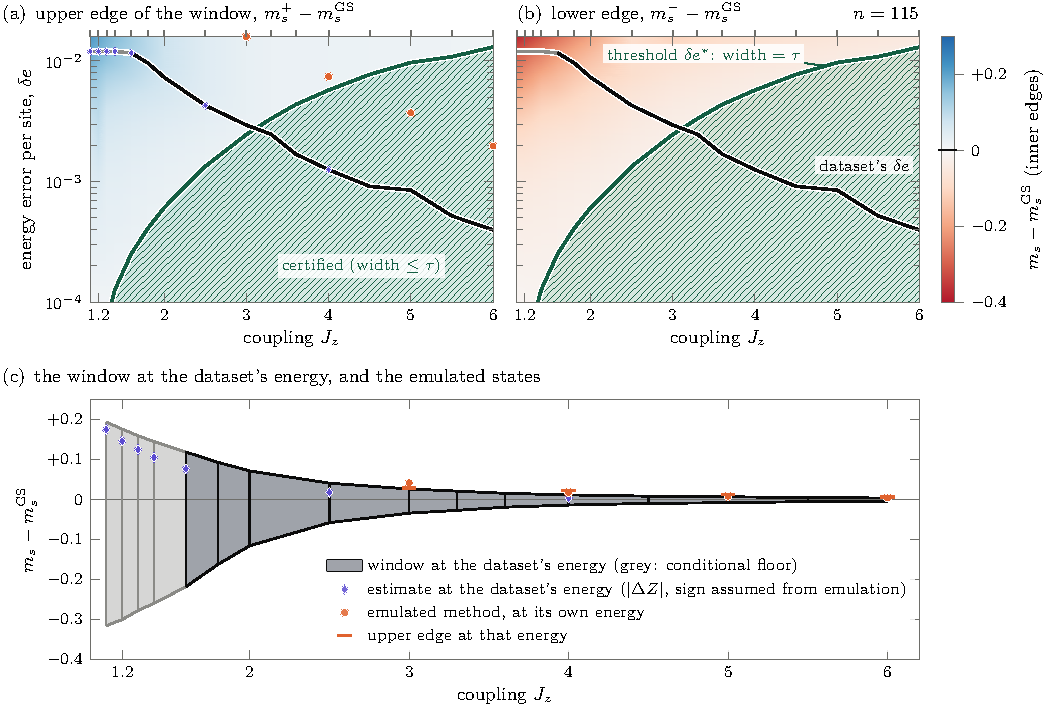
\includegraphics[width=\textwidth]{figS_landscape_n115_pgf}%
\caption{\label{fig:A_landscape115}The full certification landscape (Supplemental Fig.~S1) at $n=115$ (orange: only the emulated states with $\Jz\ge3.0$ fall inside
the plotted range). The $\de$ range stops at $0.016$, just below the highest stored energy common to all couplings % src: file:paper/figures/pgf_sm_3d/export_check.txt (0.016; 0.01663 at J_z = 2.5)
($0.0166$, set by $\Jz=2.5$). % src: file:paper/figures/pgf_sm_3d/export_check.txt (0.01663)
At $\Jz=3.0$ the emulated state ($+0.042$) lies above the drawn upper edge at its energy ($+0.029$): % src: file:paper/figures/pgf_sm_3d/export_check.txt (0.0417, 0.0287); derived: 0.0417 -> 0.042 and 0.0287 -> 0.029 (rounded)
the edges are inner, built from the stored states, and bound the true edges from inside. At this size the emulation
does not reach the dataset's energy quality (Supplemental Sec.~S5). Source: deposited map and method outputs.}
\end{figure}

\begin{figure}[h]
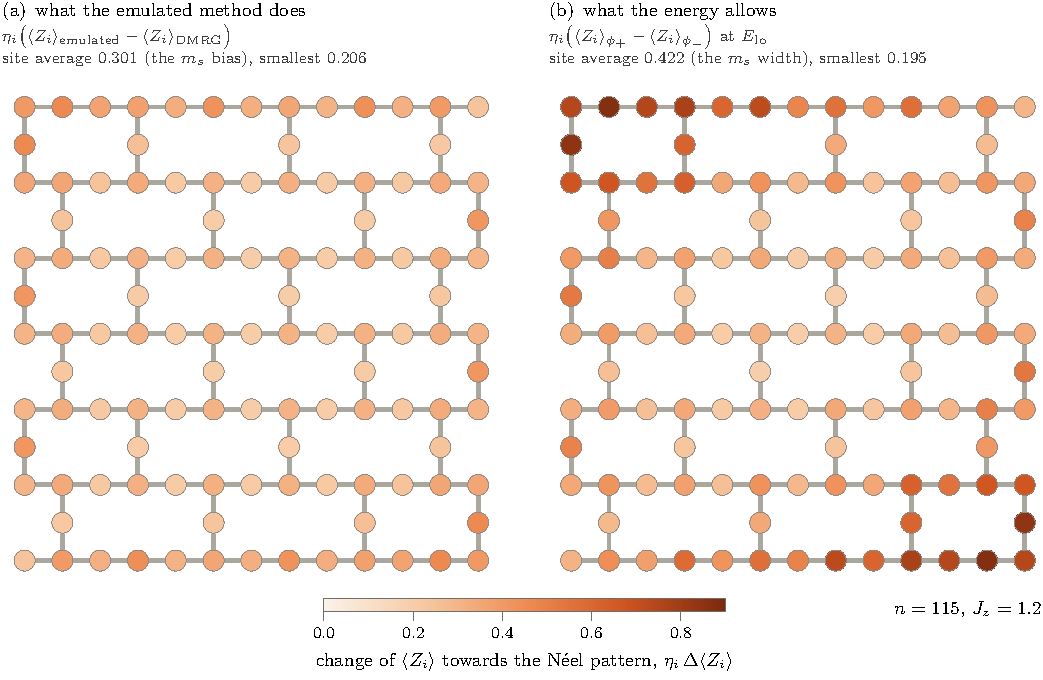
\includegraphics[width=\textwidth]{figS_lattice_n115_pgf}%
\caption{\label{fig:A_lattice115}Site by site at $\Jz=1.2$ (as Supplemental Fig.~S2) at $n=115$, where the emulation does not reach the dataset's energy quality
(Supplemental Sec.~S5; emulated state at $\de=0.079$, witnesses at $0.0096$). Every site is again more ordered in the % src: file:paper/figures/pgf_sm_3d/export_check.txt (0.079 = 0.07865; 0.0096); derived: 0.8 x 0.012 = 0.0096
emulated state, and the freedom left by the energy is greatest near two corners of the lattice.}
\end{figure}

\end{document}
